\documentclass[]{beamer}
\usetheme{Frankfurt}
\setbeamertemplate{footline}[frame number]
% Class options include: notes, notesonly, handout, trans,
%                        hidesubsections, shadesubsections,
%                        inrow, blue, red, grey, brown

% Theme for beamer presentation.

\usepackage{datetime}
\usepackage{layouts}
\usepackage{layout}
\RequirePackage{lmodern}
\RequirePackage[T1]{fontenc}
\RequirePackage[utf8]{inputenc}
\RequirePackage{microtype}
\RequirePackage{eurosym}
\usepackage{layouts}
\usepackage{layout}
\usepackage{algorithm}
\usepackage{algpseudocode}

%----------------------------------------------------------------%
% MATH                                                           %
\RequirePackage{amssymb}
\RequirePackage{amsmath}
\RequirePackage{amsfonts} 
\RequirePackage{bm}
\RequirePackage{mathtools}
\RequirePackage{dcolumn}
\RequirePackage{nicefrac}
\RequirePackage{siunitx}

%----------------------------------------------------------------%

%----------------------------------------------------------------%
% Figures, tables                                                %
\RequirePackage{graphicx}
\RequirePackage{float}
\RequirePackage{multicol}
\RequirePackage{multirow}
\RequirePackage{array}
\RequirePackage{xcolor}
\RequirePackage{wrapfig}
\RequirePackage{placeins}
\RequirePackage{bbm}
\RequirePackage[hang,bf]{caption}
\RequirePackage{etoolbox}
\RequirePackage{tabularx}
\RequirePackage{paralist}
\RequirePackage{subfigure}
%----------------------------------------------------------------%

%----------------------------------------------------------------%
% Other packages                                                 %
\RequirePackage{fancyhdr}
\RequirePackage{lastpage}
\RequirePackage{pdfpages}
\RequirePackage{natbib}
\RequirePackage{nicefrac}
\RequirePackage{amsthm}
\RequirePackage{thmtools}
\RequirePackage{needspace}
\newcommand{\dif}[2]{\ensuremath{\frac{\mathrm{d}\, #1}{\mathrm{d}\, #2}}}
\newcommand{\diff}[2]{\ensuremath{\frac{\partial\, #1}{\partial\, #2}}}
\newcommand{\lrp}[1]{\ensuremath{\left( #1 \right)}}
\newcommand{\ui}[2]{#1 _{\text{#2}}}
\newdateformat{monthyeardate}{%
	\monthname[\THEMONTH], \THEYEAR}
% Other themes include: beamerthemebars, beamerthemelined, 
%                       beamerthemetree, beamerthemetreebars  

\title{Nonlinear Model Predictive Control\\ of Rotary Inverted Pendulum}    % Enter your title between curly braces
\subtitle{MASTER THESIS}
\author{Bc. Alexey Morozov}                 % Enter your name between curly braces
\institute{\footnotesize{ SLOVAK UNIVERSITY OF TECHNOLOGY IN BRATISLAVA\\ FACULTY OF CHEMICAL AND FOOD TECHNOLOGY\\lInstitute of Information Engineering, Automation, and Mathematics}}      % Enter your institute name between curly braces
\author{Bc. Alexey Morozov} 
\date{\monthyeardate\today}                    % Enter the date or \today between curly braces
\usepackage{sidecap}
\makeatletter
\newcommand\titlegraphicii[1]{\def\inserttitlegraphicii{#1}}
\titlegraphicii{}
\setbeamertemplate{title page}
{
	{\usebeamercolor[fg]{titlegraphic}\inserttitlegraphic\hfill\inserttitlegraphicii\par}
	\begin{centering}
		\begin{beamercolorbox}[sep=8pt,center]{institute}
			\usebeamerfont{institute}\insertinstitute
		\end{beamercolorbox}
	\vskip0.5em
		\begin{beamercolorbox}[sep=8pt,center]{title}
			\usebeamerfont{title}\inserttitle\par%
			\ifx\insertsubtitle\@empty%
			\else%
			\vskip0.5em%
			{\usebeamerfont{subtitle}\usebeamercolor[fg]{subtitle}\insertsubtitle\par}%
			\fi%     
		\end{beamercolorbox}%
		\vskip2em\par
		\begin{beamercolorbox}[sep=8pt,center]{author}
			\usebeamerfont{author}\insertauthor
		\end{beamercolorbox}
	\vskip1em
	\end{centering}
	%\vfill
}
\makeatother
\definecolor{mygray}{gray}{0.7}

\begin{document}
\beamertemplatenavigationsymbolsempty
% Creates title page of slide show using above information

\begin{frame}[plain]
	\maketitle
	\small
	\vskip1em
	\begin{columns}[c]
		\column{0.6\textwidth}

		\begin{tabular}[t]{@{}l@{\hspace{3pt}}p{.6\textwidth}@{}}
			Supervisor: & Ing. Martin Klaučo, PhD. 
		\end{tabular}%
		\column{0.4\textwidth}

		\begin{tabular}[t]{@{}l@{\hspace{3pt}}p{.6\textwidth}@{}}
			Consultant: & Ing. Matúš Furka
		\end{tabular}%
	\end{columns}
	\normalsize
	\vskip2.5em
	\centering\insertdate
\end{frame}

\section{Intro}                          


\subsection{Rotatry Inverted Pendulum}
\begin{frame}
  \frametitle{Furuta Pendulum Device}
   	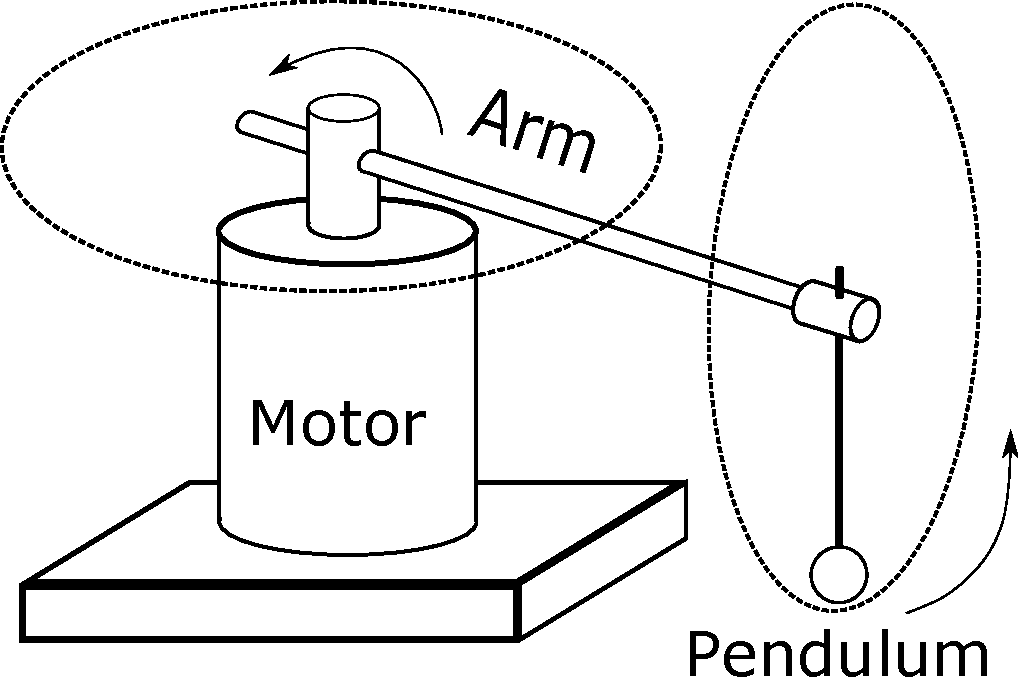
\includegraphics[scale=0.6]{images/furuta1.pdf}
\end{frame}


\subsection{Control Objective}
\begin{frame}
  \frametitle{Swing-Up Control of the Pendulum}
  \centering 
  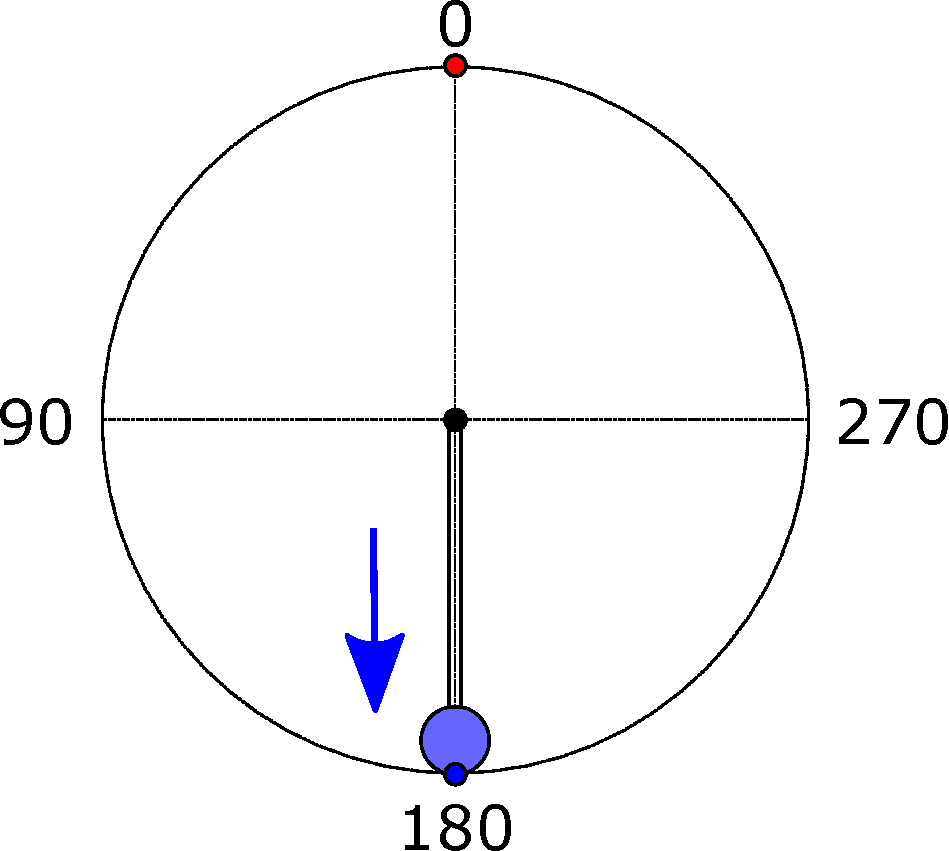
\includegraphics[scale=0.5]{images/OP2.pdf}
\end{frame}
\begin{frame}
	\frametitle{Swing-Up Control of the Pendulum}
	\centering 
	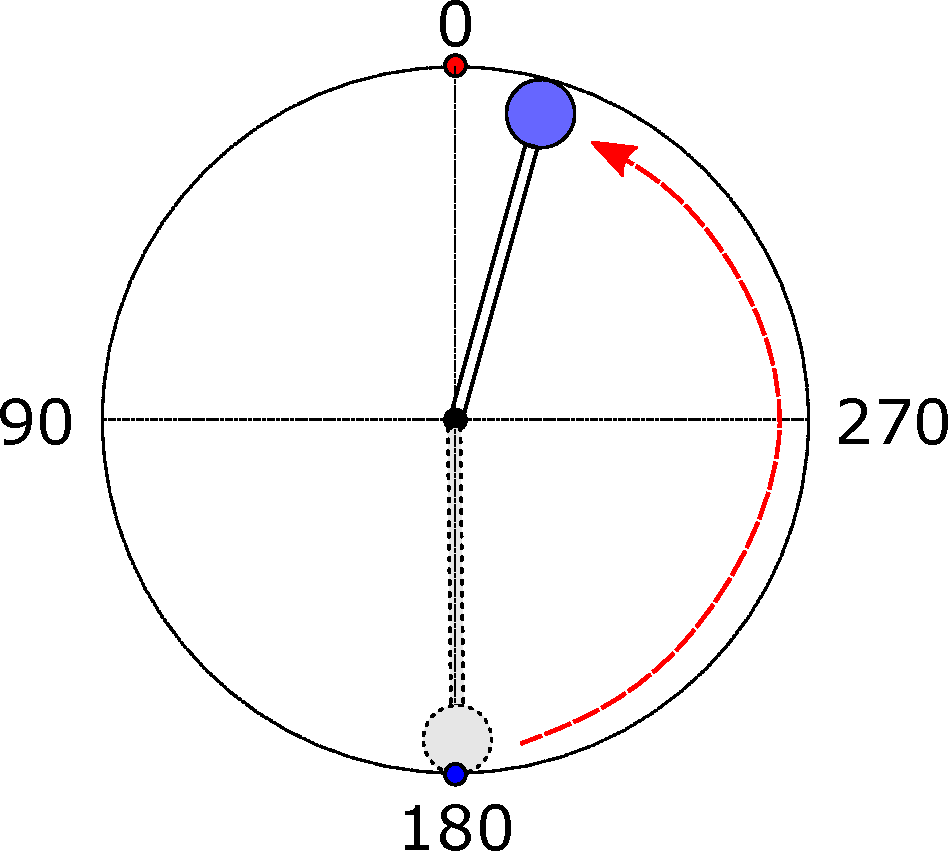
\includegraphics[scale=0.5]{images/OP3.pdf}
\end{frame}
\begin{frame}
	\frametitle{Swing-Up Control of the Pendulum}
	\centering 
	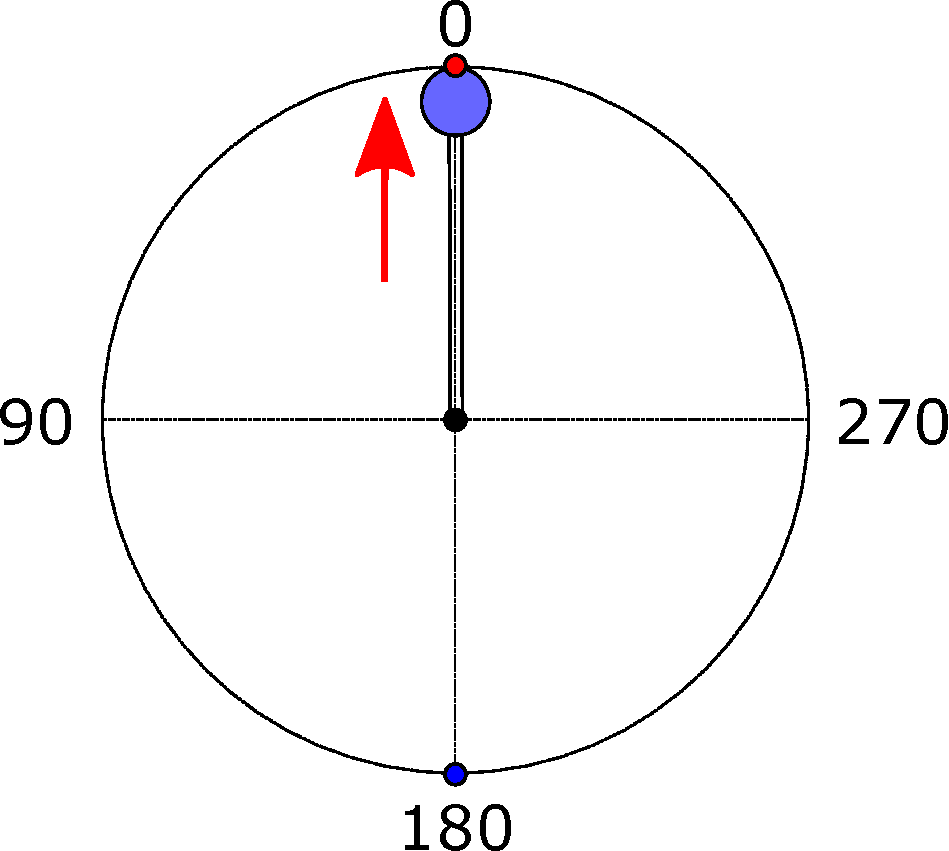
\includegraphics[scale=0.5]{images/OP4.pdf}
\end{frame}

\begin{frame}
	\frametitle{Swing-Up Control of the Pendulum}	
		\begin{columns}[c]	
		\column{0.6\textwidth}
		Main control strategies
		\begin{enumerate}
			\item Heuristic Swing-Up Control strategy\\
			\item Optimal Swing-Up Control strategy
		\end{enumerate}
	\column{0.4\textwidth}
	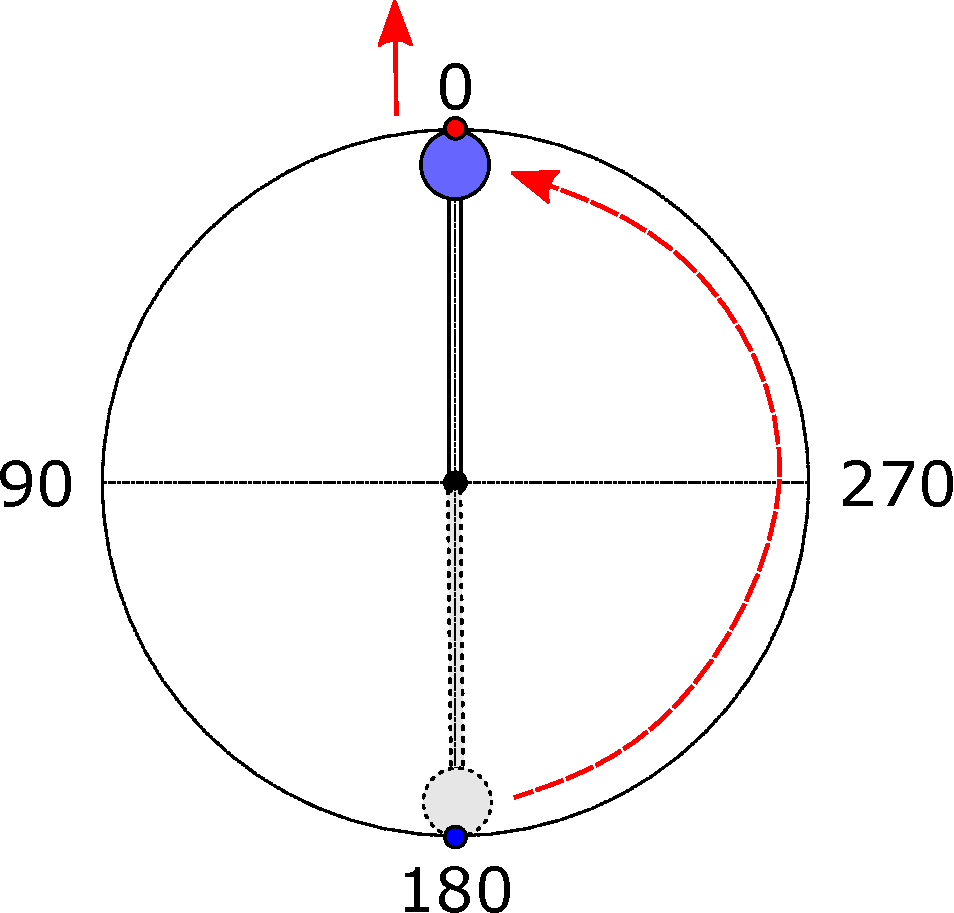
\includegraphics[scale=0.29]{images/OP_total.pdf}
\end{columns}
\end{frame}

\section{Furuta Pendulum}
\begin{frame}
	\frametitle{Furuta Pendulum Device}
	\centering
	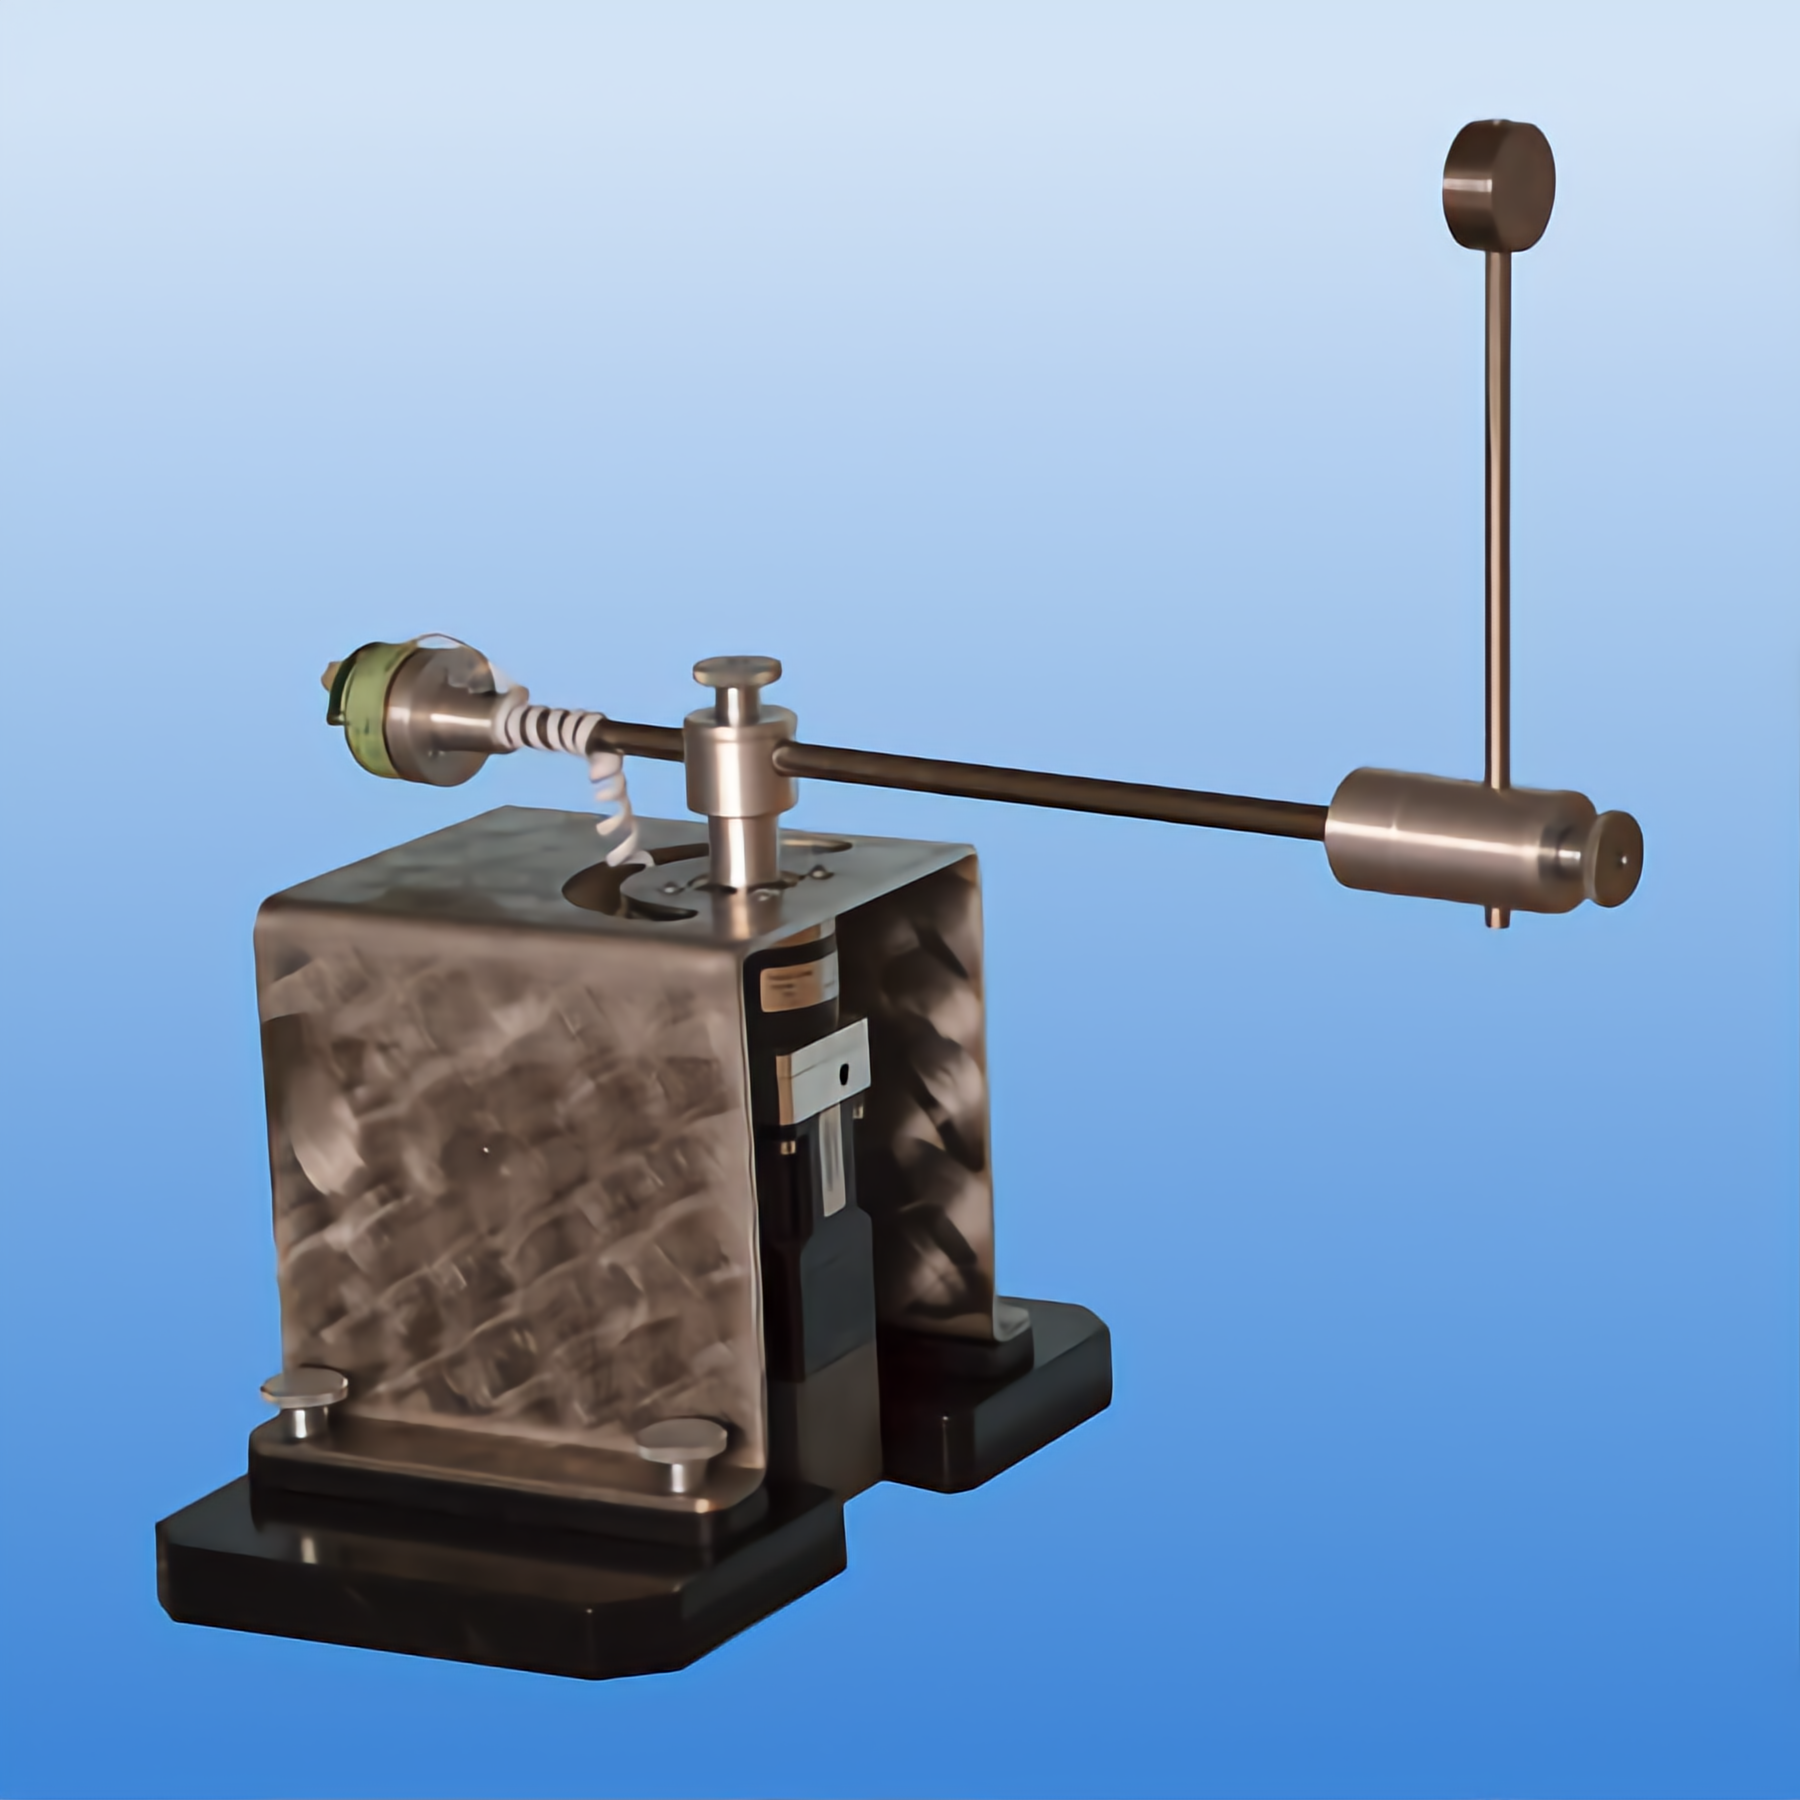
\includegraphics[scale=0.5]{images/furutareal.png}
\end{frame}
\subsection{Mathematical Model}

\begin{frame}
	\frametitle{Derivation of the Mathematical Model}
	\framesubtitle{Lagrangian Formulation}
Lagrangian
\begin{equation*}
L = \ui{E}{k} - \ui{E}{p}
\end{equation*}
Euler-Lagrange Equations
\begin{subequations}
	\begin{align*}
	\dif{}{t}\lrp{\diff{L}{\dot{\theta}_0}}-\diff{L}{\dot{\theta}_0} = \tau\\
	\dif{}{t}\lrp{\diff{L}{\dot{\theta}_1}}-\diff{L}{\dot{\theta}_1} = 0
	\end{align*}
\end{subequations}
\end{frame}
\begin{frame}
	\frametitle{Derivation of the Mathematical Model}
	\framesubtitle{Lagrangian Formulation}
	Equations of motion
	\begin{subequations}
		\begin{align*}
		\ddot{\theta}_0 &= \frac{\gamma(\epsilon\dot{\theta}_0^2+\rho)-\delta(\tau+\beta\dot{\theta}_1^2-\sigma\dot{\theta}_0\dot{\theta}_1)}{\gamma^2-\alpha\delta}\\
		\ddot{\theta}_1 &= \frac{\gamma(\tau+\beta\dot{\theta}_1^2-\sigma\dot{\theta}_0\dot{\theta}_1)-\alpha(\epsilon\dot{\theta}_0^2+\rho)}{\gamma^2-\alpha\delta}
		\end{align*}
	\end{subequations}
Parametres
\begin{subequations}
	\begin{align*}
	\alpha &= I_0+L_0^2m_1+l_1^2m_1\sin^2\theta_1\\
	\beta &= L_0m_1l_1\sin\theta_1 \\
	\gamma &= L_0m_1l_1\cos\theta_1\\
	\delta &= I_1+l_1^2m_1\\
	\epsilon &= l^2_1m_1\sin\theta_1\cos\theta_1\\
	\rho &= m_1gl_1\sin\theta_1\\
	\sigma &= 2l^2_1m_1\sin\theta_1\cos\theta_1
	\end{align*}
\end{subequations}
\end{frame}
\begin{frame}
	\frametitle{Derivation of the Mathematical Model}
	\framesubtitle{State-Space Formulation}
	  	\begin{columns}[c]
		\column{2in}  % slides are 3in high by 5in wide
State variables
\begin{equation*}
\begin{bmatrix}
x_1(t)\\x_2(t)\\x_3(t)\\x_4(t)
\end{bmatrix} = \begin{bmatrix}
\theta_0(t)\\\dot{\theta}_0(t)\\\theta_1(t)\\\dot{\theta}_1(t)
\end{bmatrix}
\end{equation*}
Control input
\begin{equation*}
u(t) = \tau (t)
\end{equation*}
		\column{2in}
		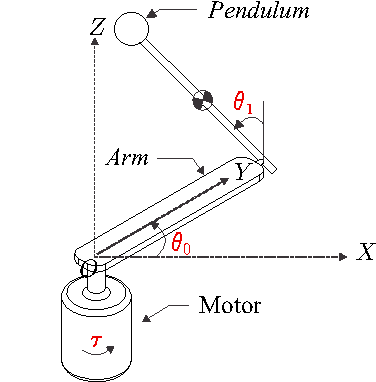
\includegraphics[scale=0.55]{images/furuta2.png}
	\end{columns}
\end{frame}
\begin{frame}
	\frametitle{Derivation of the Mathematical Model}
	\framesubtitle{State-Space Formulation}
	Non-linear model
	\begin{equation*}
	\begin{bmatrix}
	\dot{x}_1(t) \\ \dot{x}_2(t) \\ \dot{x}_3(t) \\ \dot{x}_4(t)
	\end{bmatrix} = \begin{bmatrix}
	\dot{\theta}_0\\
	\frac{\gamma(\epsilon\dot{\theta}_0^2+\rho)-\delta(\tau+\beta\dot{\theta}_1^2-\sigma\dot{\theta}_0\dot{\theta}_1)}{\gamma^2-\alpha\delta}\\
	\dot{\theta}_1\\
	\frac{\gamma(\tau+\beta\dot{\theta}_1^2-\sigma\dot{\theta}_0\dot{\theta}_1)-\alpha(\epsilon\dot{\theta}_0^2+\rho)}{\gamma^2-\alpha\delta}
	\end{bmatrix}
	\end{equation*}
\end{frame}
\begin{frame}
	\frametitle{Derivation of the Mathematical Model}
	\framesubtitle{State-Space Formulation}
	Linear model
	\begin{subequations}
		\begin{align*}
		A &=\begin{bmatrix}0&1&0&0\\
		0&0&\frac{-gL_0l_1^2m_1^2}{(m_1L_0^2+I_0)(m_1l_1^2+I_1)-L_0^2l_1^2m_1^2}&0\\
		0&0&0&1\\
		0&0&\frac{gl_1m_1(m_1L_0^2+I_0)}{(m_1L_0^2+I_0)(m_1l_1^2+I_1)-L_0^2l_1^2m_1^2}&0
		\end{bmatrix}\\
		B &=	\begin{bmatrix}
		0\\ 
		\frac{m_1L_1^2+I_1}{(m_1L_0^2+I_0)(m_1l_1^2+I_1)-L_0^2l_1^2m_1^2}\\
		0\\
		\frac{-L_0l_1m_1}{(m_1L_0^2+I_0)(m_1l_1^2+I_1)-L_0^2l_1^2m_1^2}
		\end{bmatrix}
		\end{align*}
	\end{subequations}
\end{frame}

\section{Control of the Pendulum}

\begin{frame}
	\frametitle{Swing-Up Control of the Pendulum}	
	\begin{columns}[c]	
		\column{0.5\textwidth}
		Main control strategies
		\begin{enumerate}
			\item Heuristic Swing-Up Control strategy\\
			\item Optimal Swing-Up Control strategy
		\end{enumerate}
		\column{0.4\textwidth}
		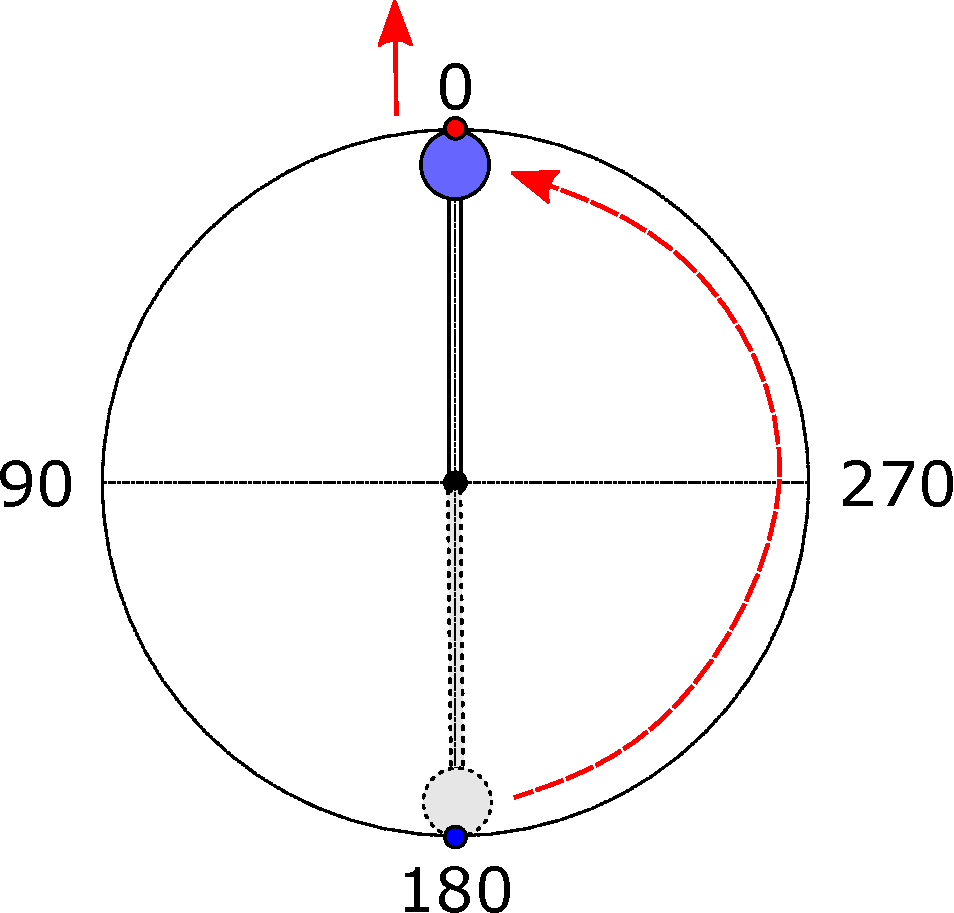
\includegraphics[scale=0.29]{images/OP_total.pdf}
	\end{columns}
\end{frame}

\subsection{Heuristic Swing-Up Control}

\begin{frame}
	\frametitle{Swing-Up Control of the Pendulum}	
	\begin{columns}[c]	
		\column{0.5\textwidth}
		Main control strategies
		\begin{enumerate}
			\item Heuristic Swing-Up Control \\strategy\\
			\item \textcolor{mygray}{Optimal Swing-Up Control\\ strategy}
		\end{enumerate}
		\column{0.4\textwidth}
		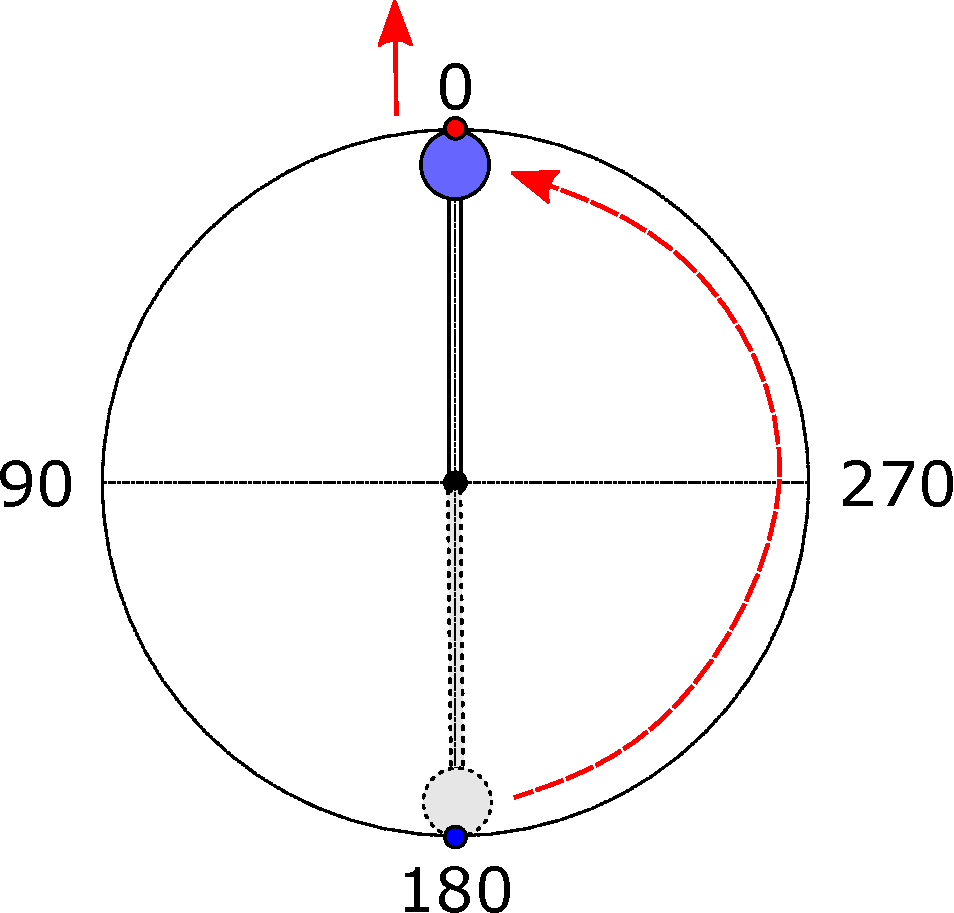
\includegraphics[scale=0.29]{images/OP_total.pdf}
	\end{columns}
\end{frame}

\begin{frame}	
	\frametitle{Heuristic Swing-Up Control}	
	\vskip0.9em
		\begin{columns}[c]	
		\column{0.6\textwidth}
	Two phases of control:
	\begin{enumerate}
		\item Initial excitation of the system\\ (by Energy-Shaping controller)\\
		\item Stabilisation of the pendulum\\(by Predictive controller)
	\end{enumerate}
		\column{0.3\textwidth}
		\end{columns}
\end{frame}	

\begin{frame}	
	\frametitle{Heuristic Swing-Up Control}	
	\vskip1.05em
	\begin{columns}[c]	
		\column{0.6\textwidth}
	Development of control strategy:
	\begin{enumerate}
		\item Design of Energy-Shaping controller\\
		\item Design of Model Predictive controller\\
		\item Full-range control of the pendulum
	\end{enumerate}
	\column{0.3\textwidth}
	\end{columns}
\end{frame}
	
\begin{frame}
	\frametitle{First Phase of Control}	
	\begin{columns}[c]	
		\column{0.5\textwidth}
		Pendulum is controlled by Energy-Shaping controller.
		\column{0.4\textwidth}
		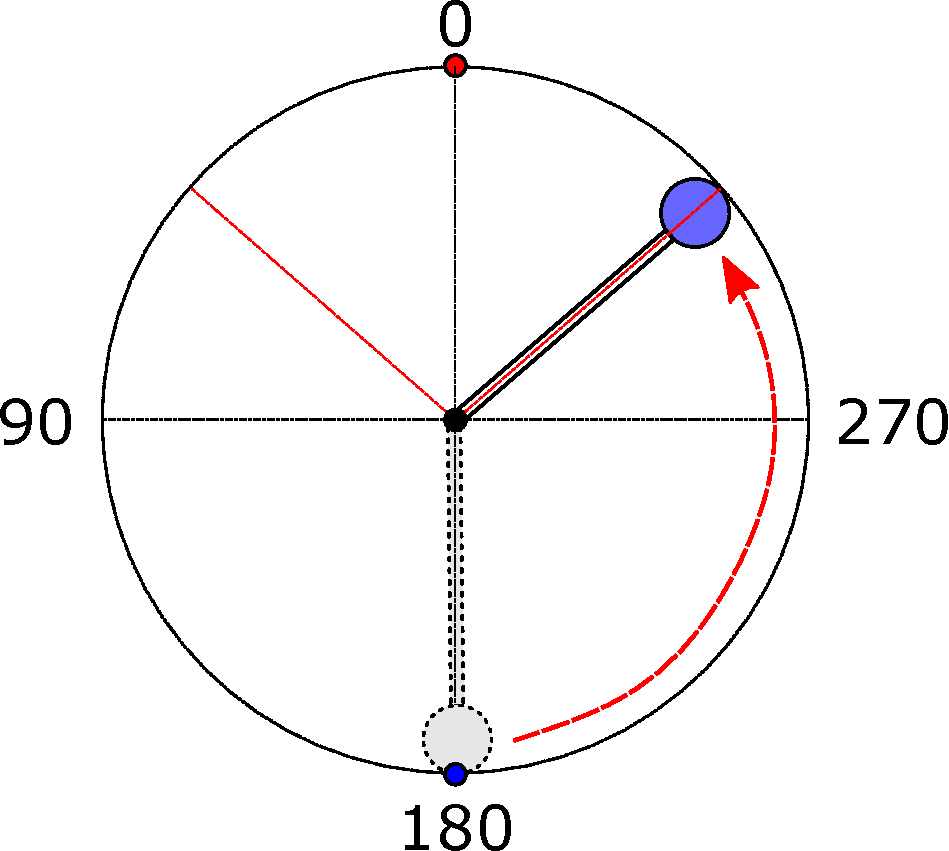
\includegraphics[scale=0.29]{images/first_phase.pdf}
	\end{columns}
\end{frame}
 
\begin{frame}
	\frametitle{First Phase of Control}
	Energy-Shaping controller
	\begin{subequations}\begin{align*}
			E &= \frac{m_1gl_1}{2}\lrp{\lrp{\frac{\dot{\theta}_1}{\omega_0}}^2+\cos(\theta_1) - 1}\\
			u &= -4E\,\text{sign}\lrp{\dot{\theta}_1\cos(\theta_1)}
		\end{align*}
	\end{subequations}
\end{frame}
\begin{frame}
	\frametitle{First Phase of Control}
	\begin{figure}[H]
		\centering
		\begin{subfigure}
			\centering
			% include first image
			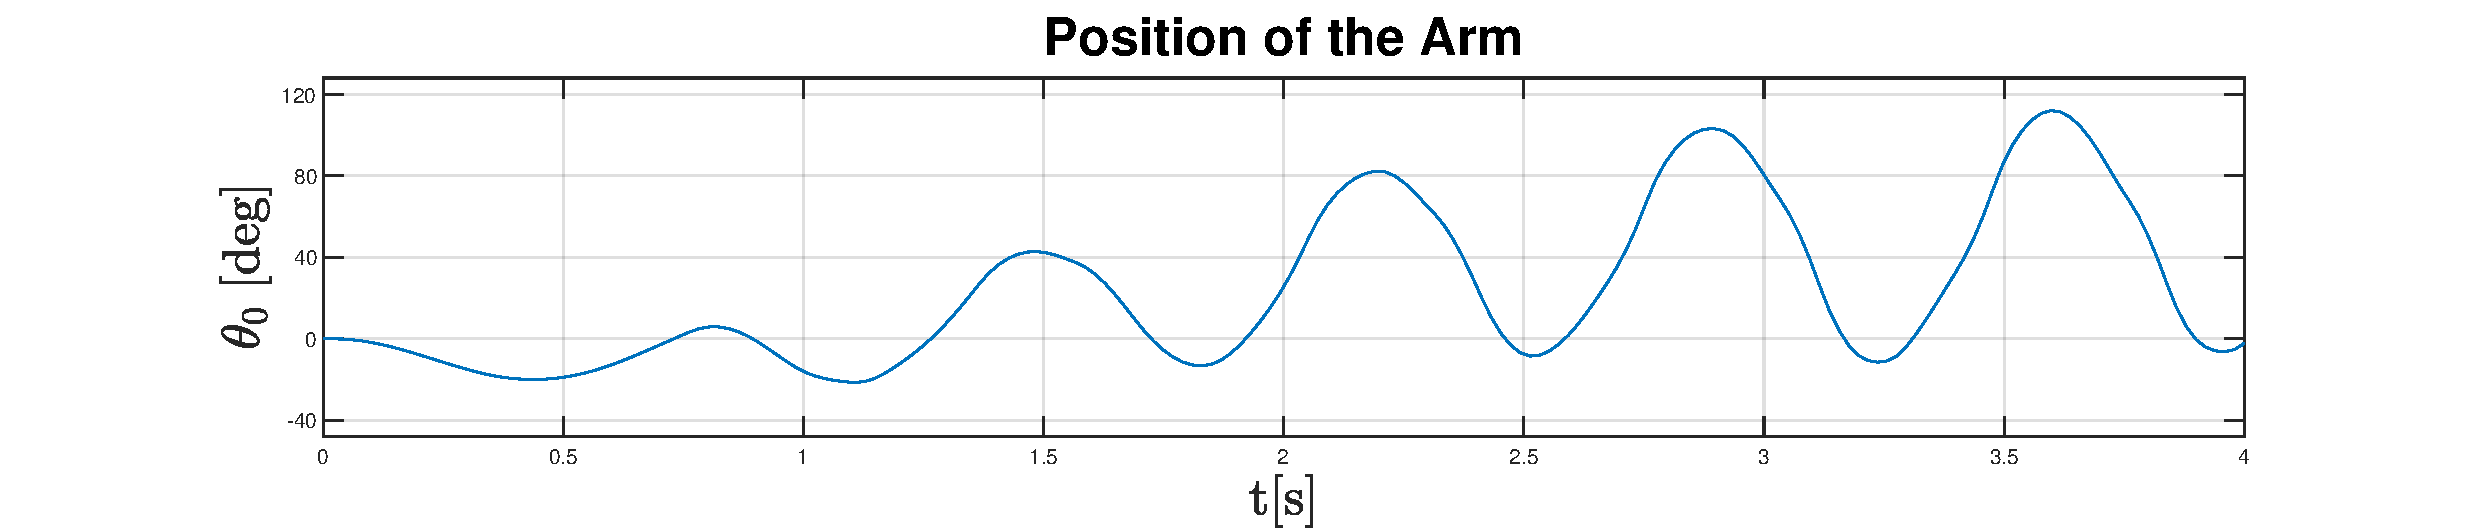
\includegraphics[scale=0.25]{images/swings/arm.pdf}  
		\end{subfigure}
		\begin{subfigure}
			\centering
			% include first image
			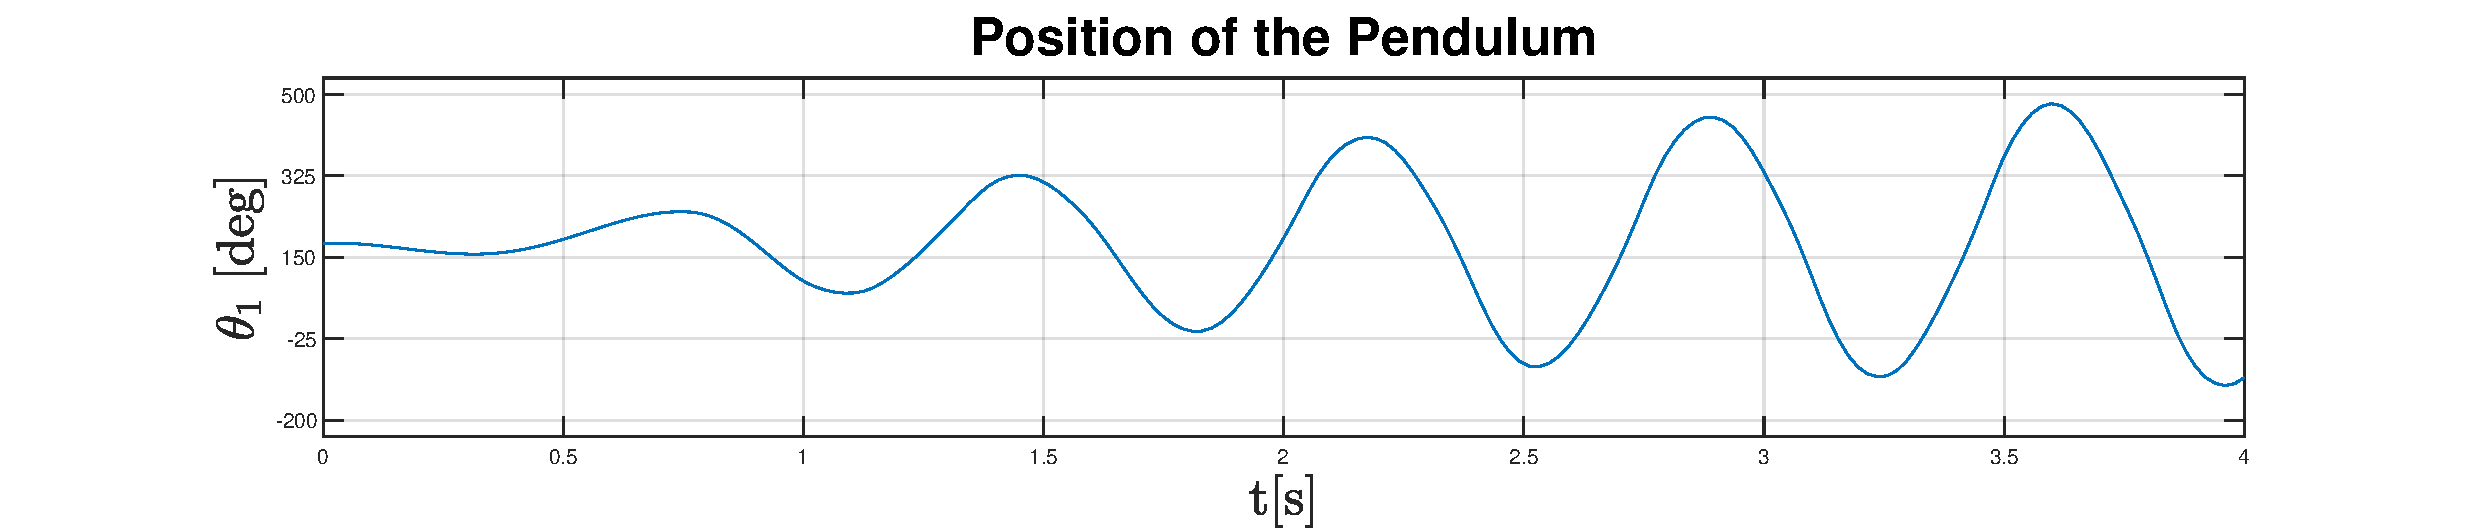
\includegraphics[scale=0.25]{images/swings/pend.pdf}  
		\end{subfigure}
		\begin{subfigure}
			\centering
			% include first image
			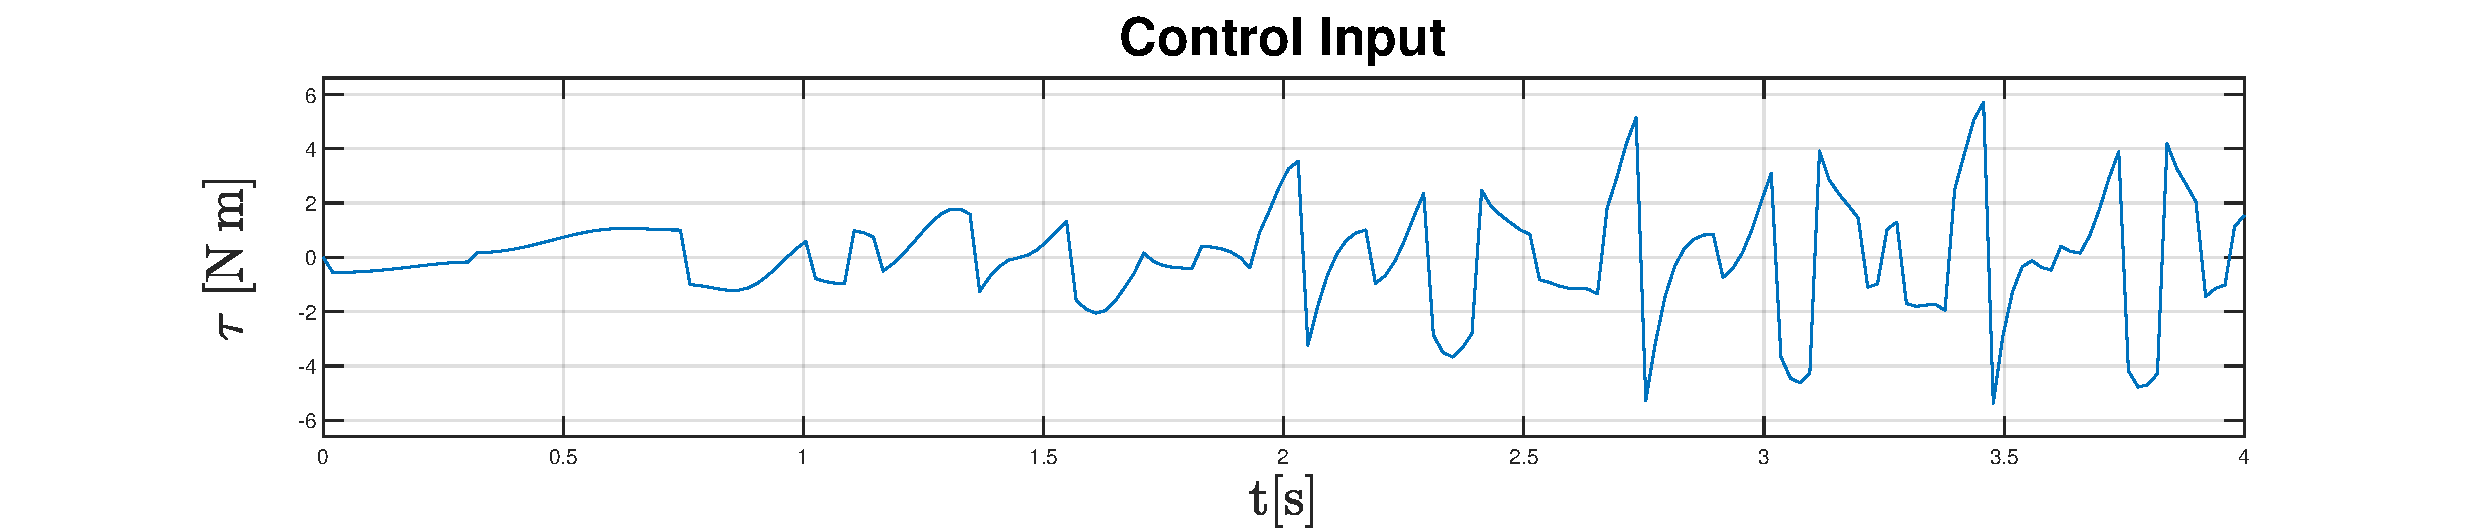
\includegraphics[scale=0.25]{images/swings/control.pdf} 
		\end{subfigure}
	\end{figure}
\end{frame}

\begin{frame}
	\frametitle{First Phase of Control}
	\begin{figure}[H]
		\centering
		\begin{subfigure}
			\centering
			% include first image
			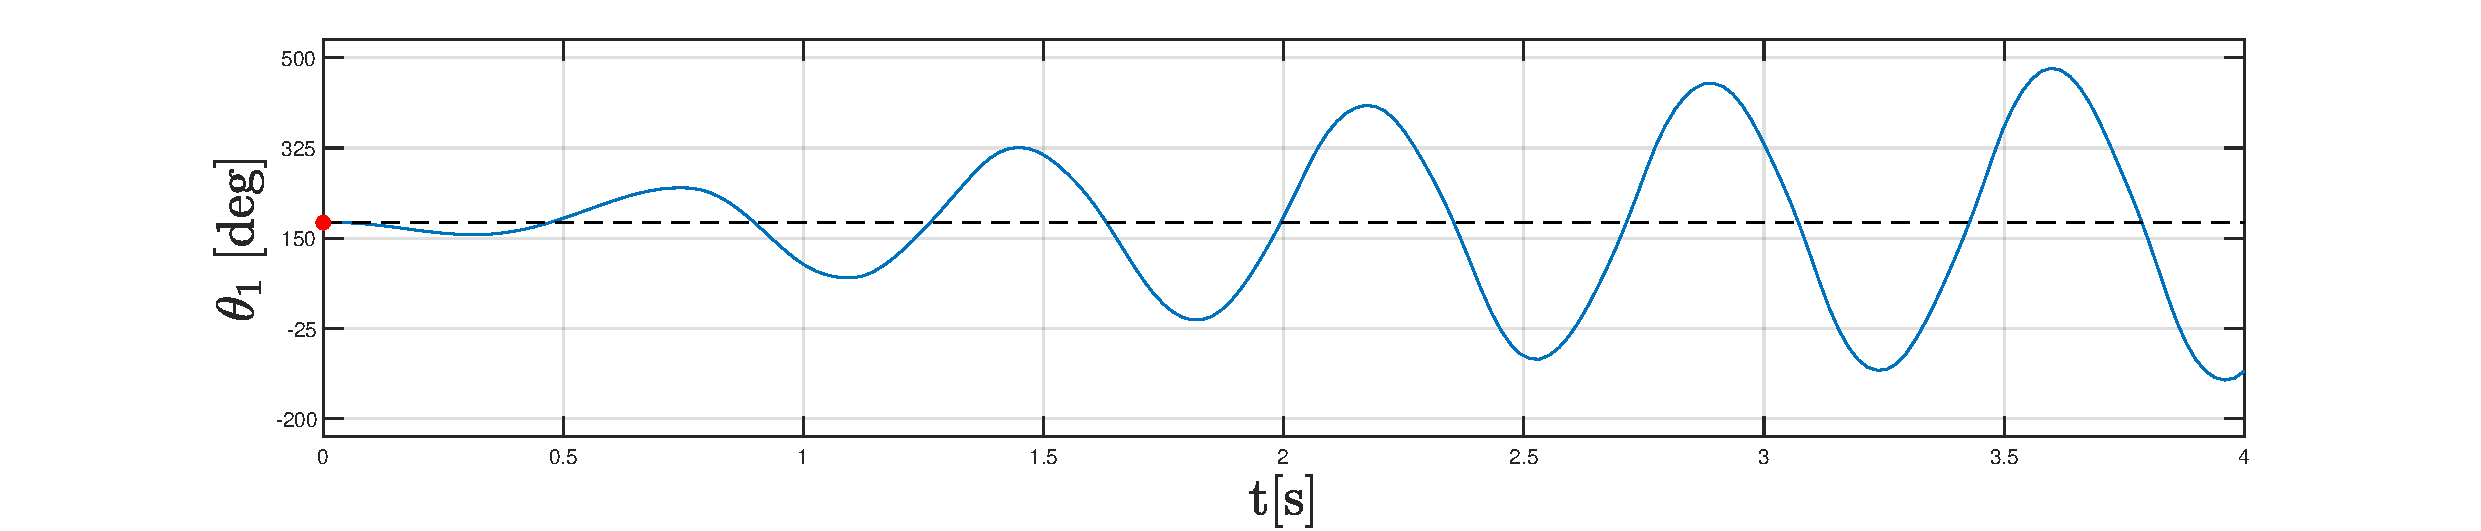
\includegraphics[scale=0.25]{images/swings2/swing1.pdf}  
		\end{subfigure}
		\begin{subfigure}
			\centering
			% include first image
			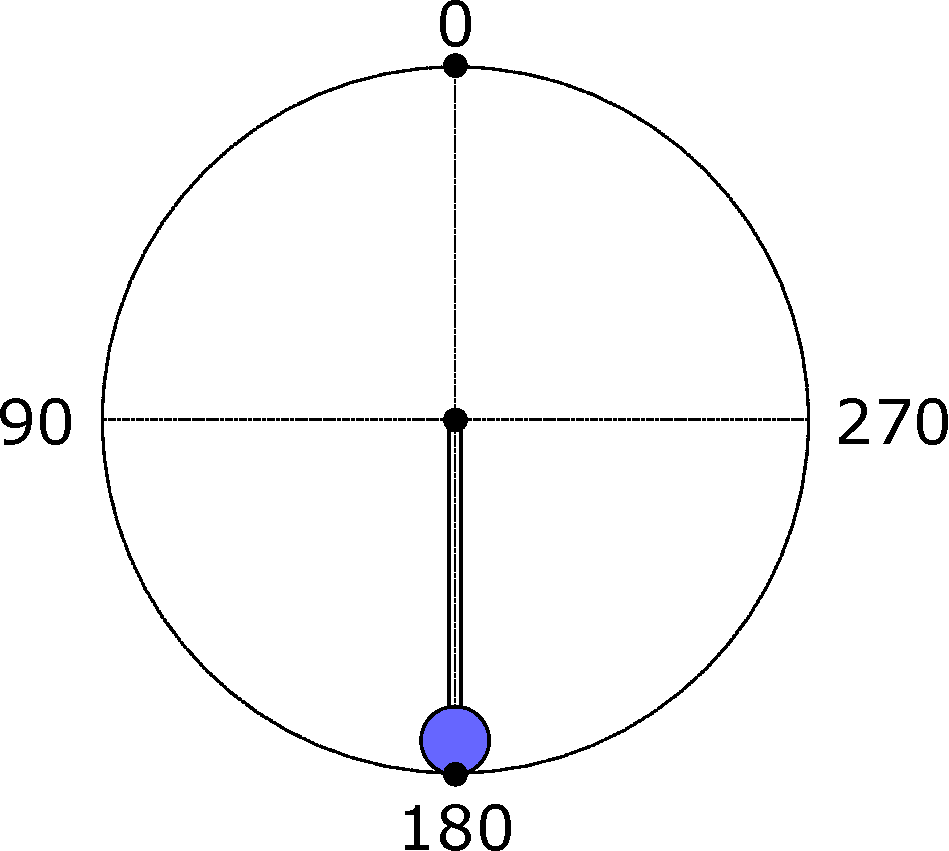
\includegraphics[scale=0.25]{images/swing0.pdf}  
		\end{subfigure}
	\end{figure}
\end{frame}

\begin{frame}
	\frametitle{First Phase of Control}
	\begin{figure}[H]
		\centering
		\begin{subfigure}
			\centering
			% include first image
			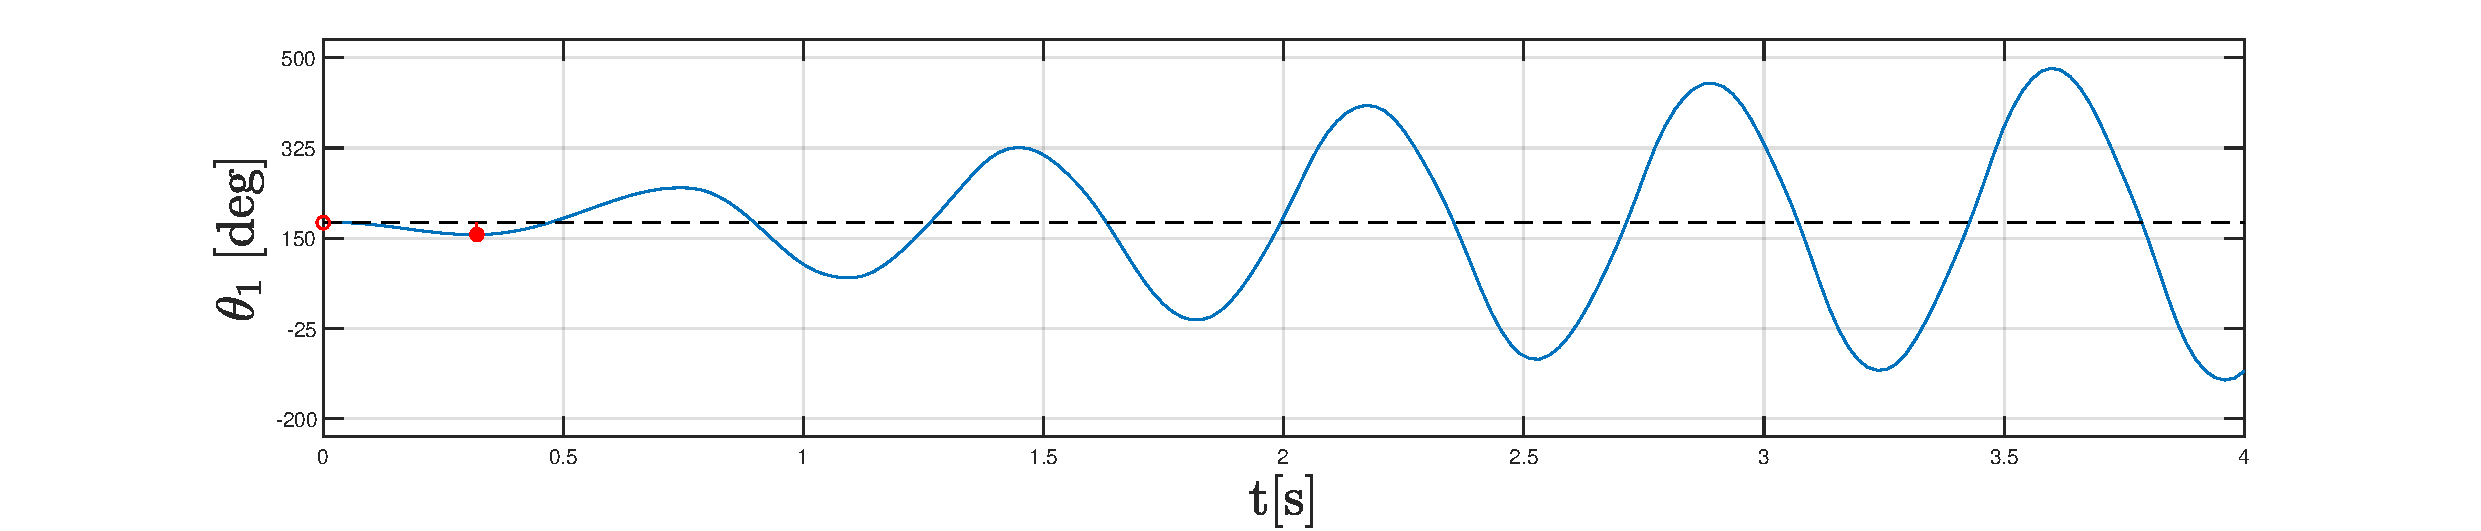
\includegraphics[scale=0.25]{images/swings2/swing2.pdf}  
		\end{subfigure}
		\begin{subfigure}
			\centering
			% include first image
			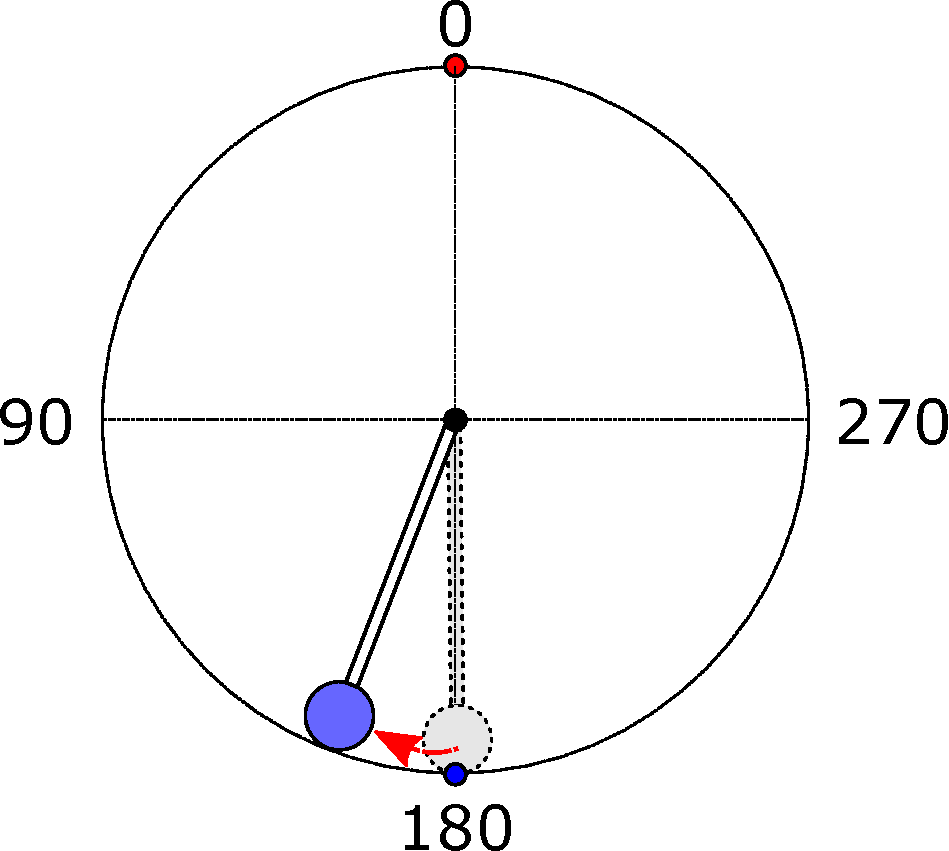
\includegraphics[scale=0.25]{images/swing1.pdf}  
		\end{subfigure}
	\end{figure}
\end{frame}

\begin{frame}
	\frametitle{First Phase of Control}
	\begin{figure}[H]
		\centering
		\begin{subfigure}
			\centering
			% include first image
			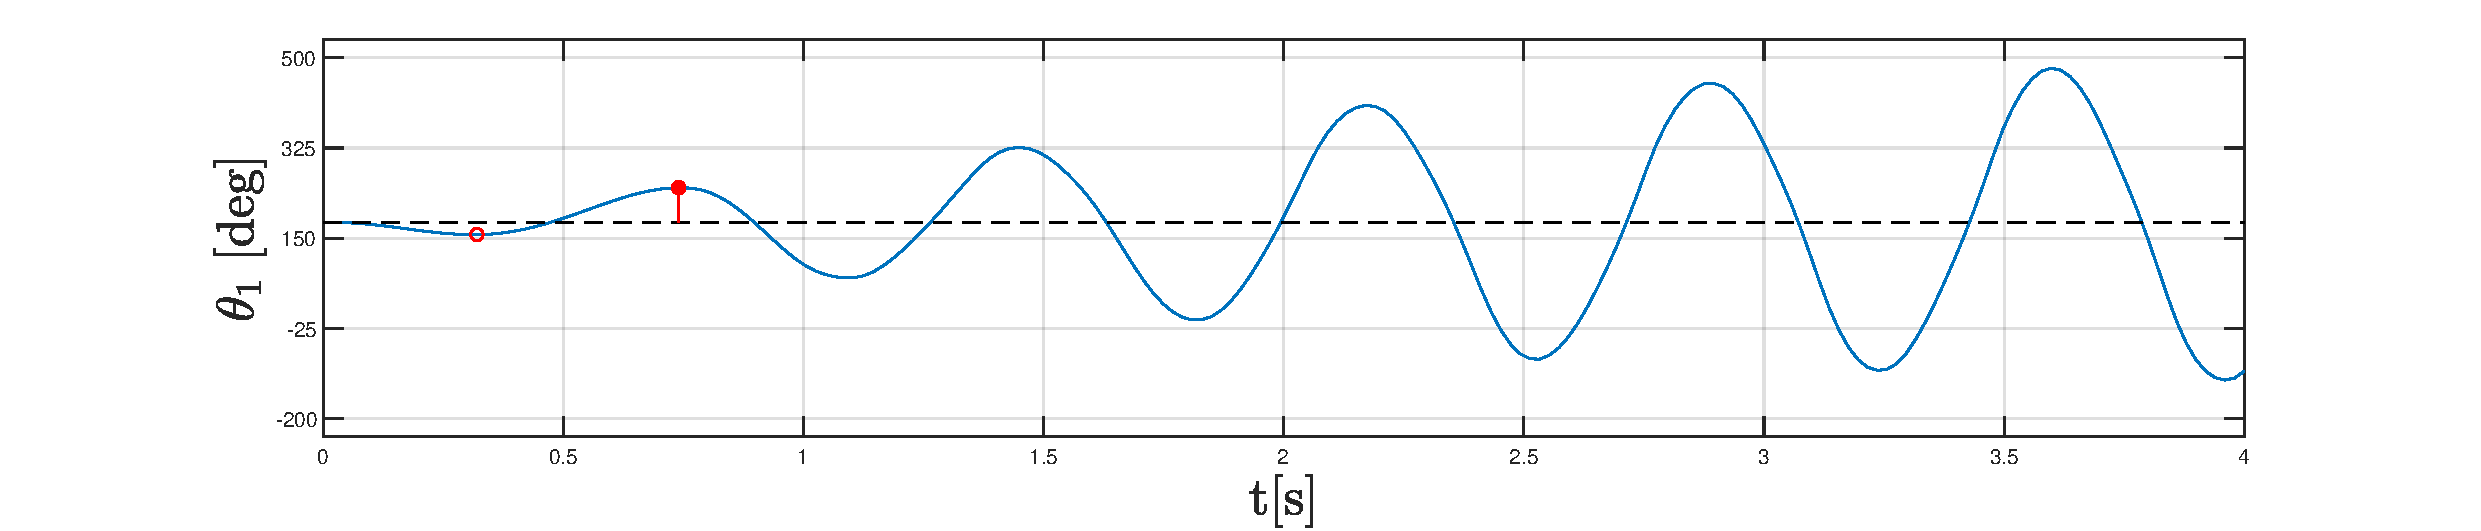
\includegraphics[scale=0.25]{images/swings2/swing3.pdf}  
		\end{subfigure}
		\begin{subfigure}
			\centering
			% include first image
			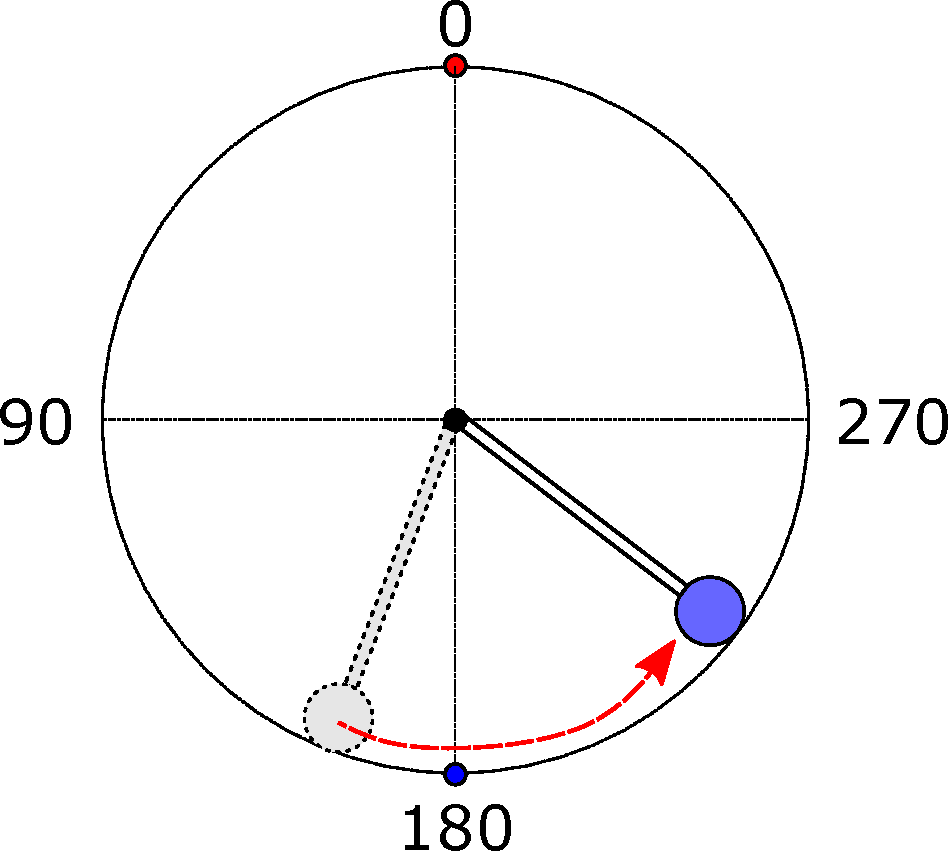
\includegraphics[scale=0.25]{images/swing2.pdf}  
		\end{subfigure}
	\end{figure}
\end{frame}

\begin{frame}
	\frametitle{First Phase of Control}
	\begin{figure}[H]
		\centering
		\begin{subfigure}
			\centering
			% include first image
			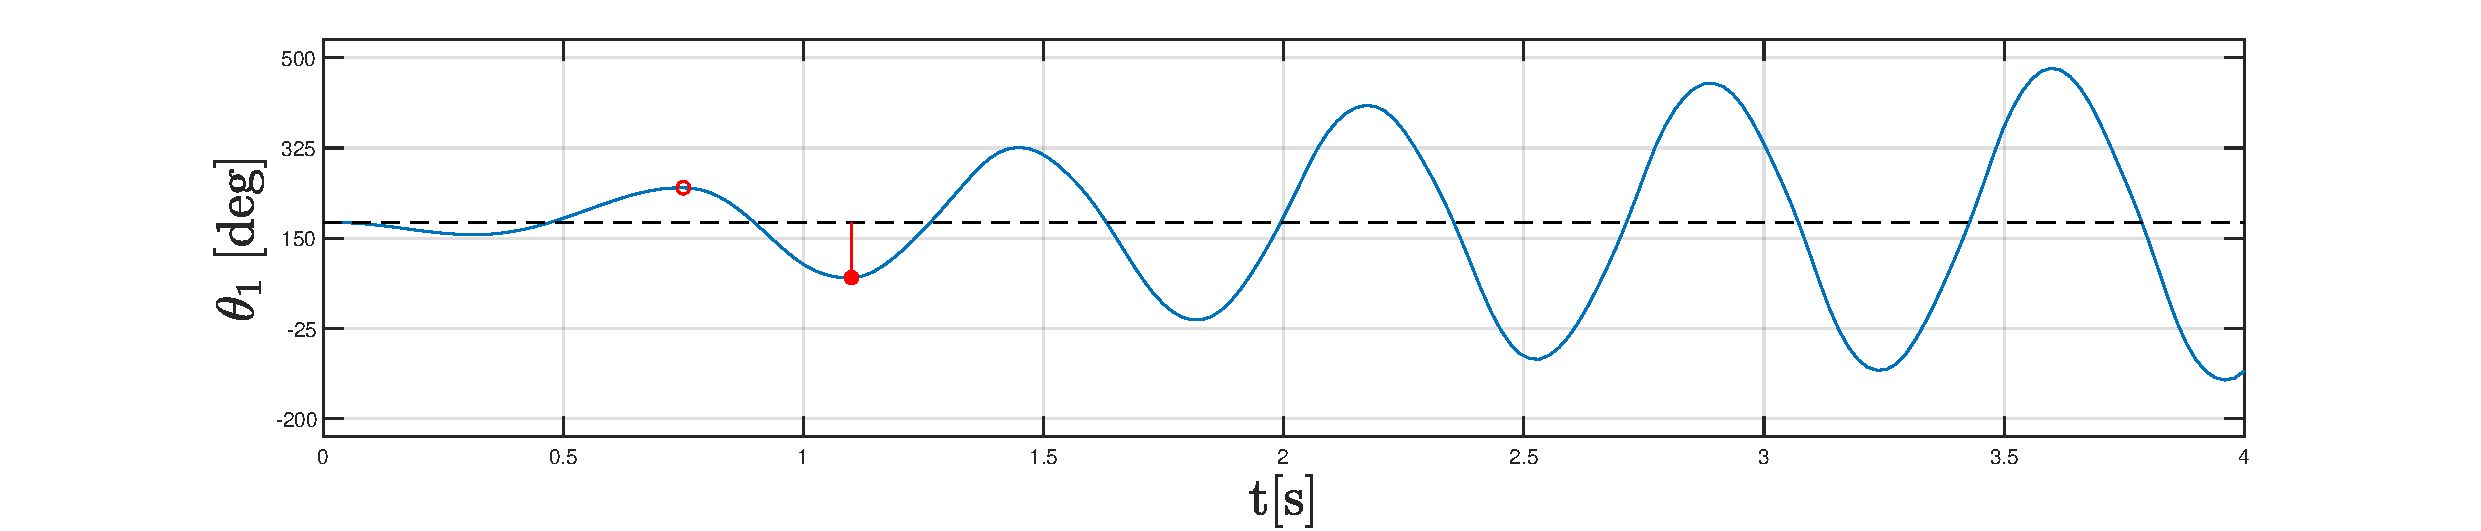
\includegraphics[scale=0.25]{images/swings2/swing4.pdf}  
		\end{subfigure}
		\begin{subfigure}
			\centering
			% include first image
			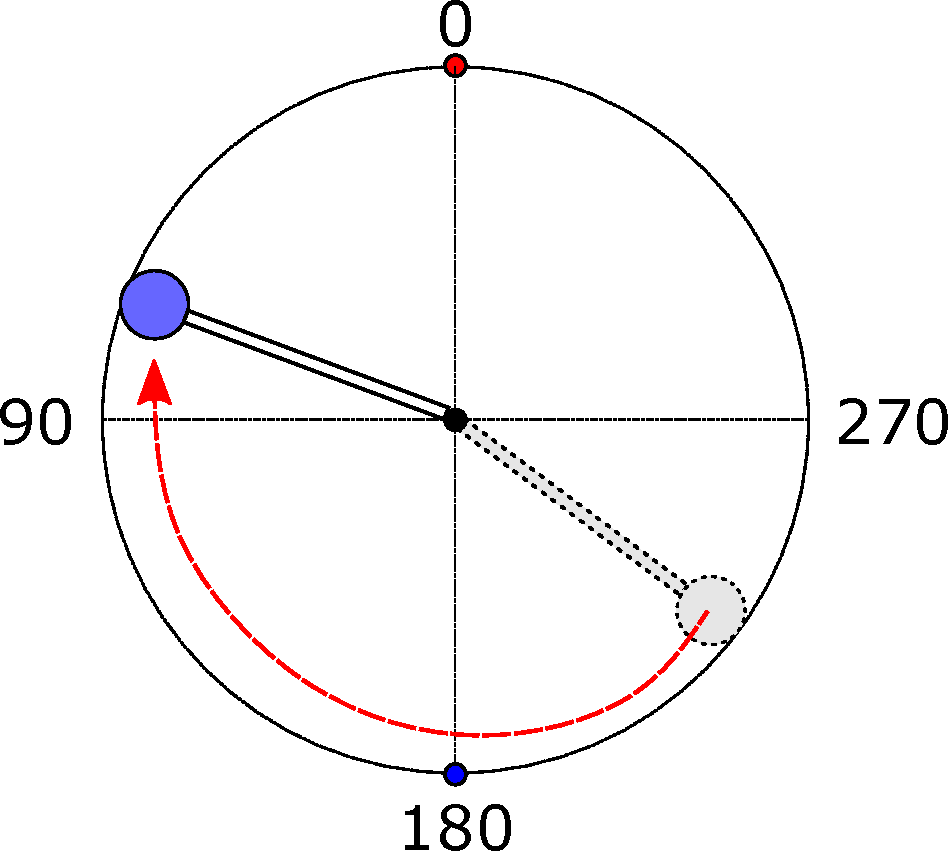
\includegraphics[scale=0.25]{images/swing3.pdf}  
		\end{subfigure}
	\end{figure}
\end{frame}

\begin{frame}
	\frametitle{Second Phase of Control}	
	\begin{columns}[c]	
		\column{0.5\textwidth}
		Pendulum is controlled by Predictive controller.
		\column{0.4\textwidth}
		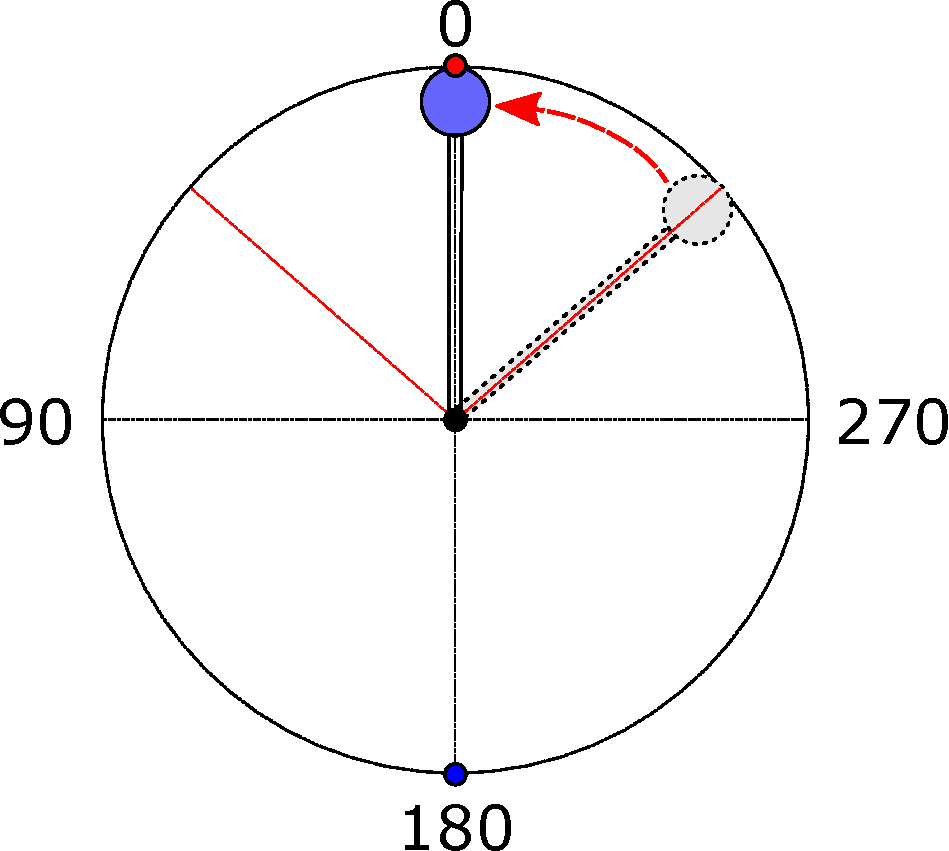
\includegraphics[scale=0.29]{images/second_phase.pdf}
	\end{columns}
\end{frame}

\begin{frame}
	\frametitle{Second Phase of Control} 
	Model Predictive Control strategy
\begin{subequations}
\begin{align*}
\min_{u_0,...,u_{N-1}}\ &\sum_{k=0}^{N-1} \lrp{ x_{k}^\intercal\ui{Q}{x}x_{k}^{\phantom{\intercal}}+u_{k}^\intercal\ui{Q}{u}u_{k}^{\phantom{\intercal}}}^{\phantom{\intercal}}\\
\text{s.t.}\quad &x_{k+1} = Ax_{k} + Bu_{k}\qquad\qquad\quad \ \   k \in \mathbb{N}_0^{N-1}\\
&\ui{u}{min}\leq u_{k}\leq \ui{u}{max}\qquad\qquad\qquad\;   k \in \mathbb{N}_0^{N-1}\\
&x_0 = x(0)		
\end{align*}
\small
	\begin{table}[H]
		\centering
		\begin{tabular}{l c c}
		\noalign{\hrule height 1pt}
		Parameter&Symbol&Value\\
		\noalign{\hrule height 1pt}
		Prediction horizon&$N$&$\ \; \,20$\\
		Initial condition&$x_0$&$\begin{bmatrix}0\ 0\ 28.5\ -40 \end{bmatrix}^\intercal$\\
		Constraint on control input-upper bound&$\ui{u}{max}$&$\ \; \,10$\\
		Constraint on control input-lower bound&$\ui{u}{min}$&$-10$\\
		\hline
	\end{tabular}
\end{table}
\end{subequations}
\end{frame}

\begin{frame}
	\frametitle{Second Phase of Control} 
	Model Predictive Control strategy
	\begin{subequations}
		\begin{align*}
			\min_{u_0,...,u_{N-1}}\ &\sum_{k=0}^{N-1} \lrp{ x_{k}^\intercal\ui{Q}{x}x_{k}^{\phantom{\intercal}}+u_{k}^\intercal\ui{Q}{u}u_{k}^{\phantom{\intercal}}}^{\phantom{\intercal}}\\
		\text{s.t.}\quad &x_{k+1} = Ax_{k} + Bu_{k}\qquad\qquad\quad \ \   k \in \mathbb{N}_0^{N-1}\\
		&\ui{u}{min}\leq u_{k}\leq \ui{u}{max}\qquad\qquad\qquad\;   k \in \mathbb{N}_0^{N-1}\\
		&x_0 = x(0)		
		\end{align*}
	\end{subequations}
Weight matrices
\begin{equation*}
\ui{Q}{x} = \begin{bmatrix}
5&0&0&0\\
0&0.08&0&0\\
0&0&10&0\\
0&0&0&0.2
\end{bmatrix} \quad \ui{Q}{u} = \num{1e-3}
\end{equation*}
\end{frame}	

\begin{frame}
	\frametitle{Second Phase of Control}
	\begin{figure}[H]
		\centering
		\begin{subfigure}
			\centering
			% include first image
			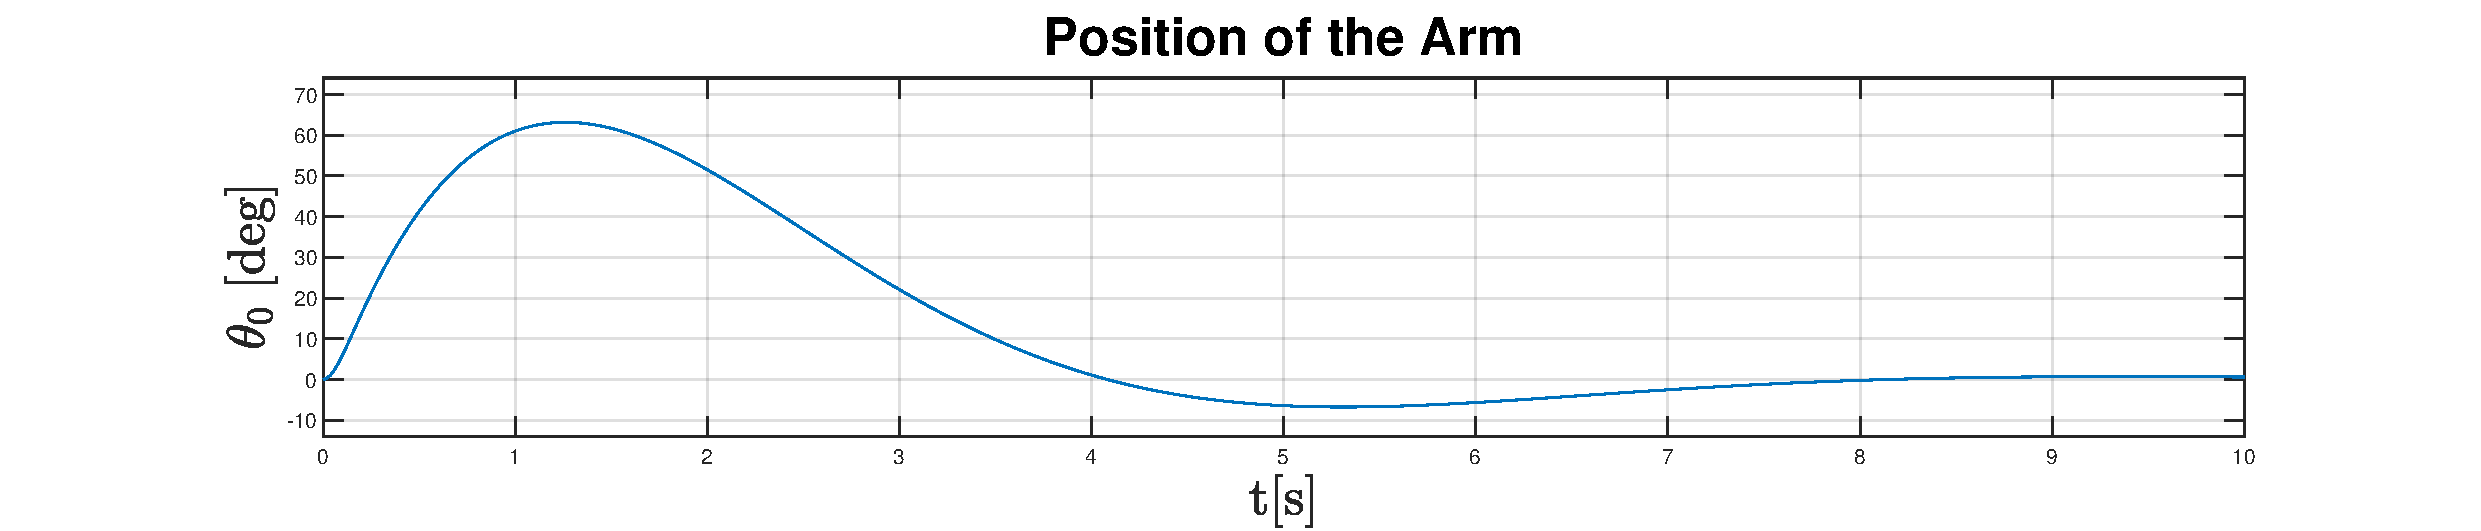
\includegraphics[scale=0.25]{images/MPC/arm.pdf}  
		\end{subfigure}
		\begin{subfigure}
			\centering
			% include first image
			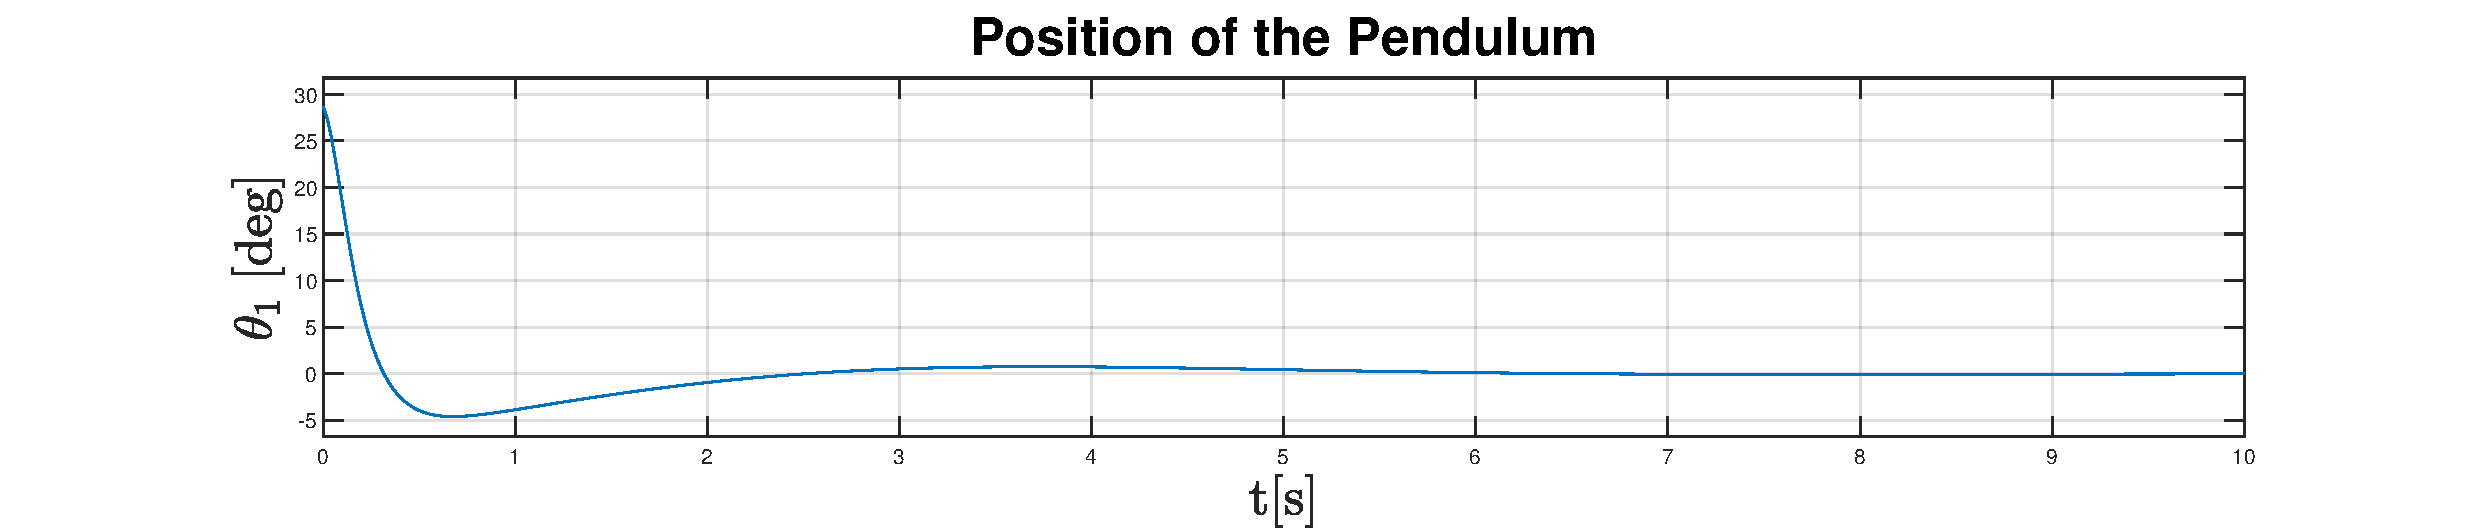
\includegraphics[scale=0.25]{images/MPC/pend.pdf}  
		\end{subfigure}
		\begin{subfigure}
			\centering
			% include first image
			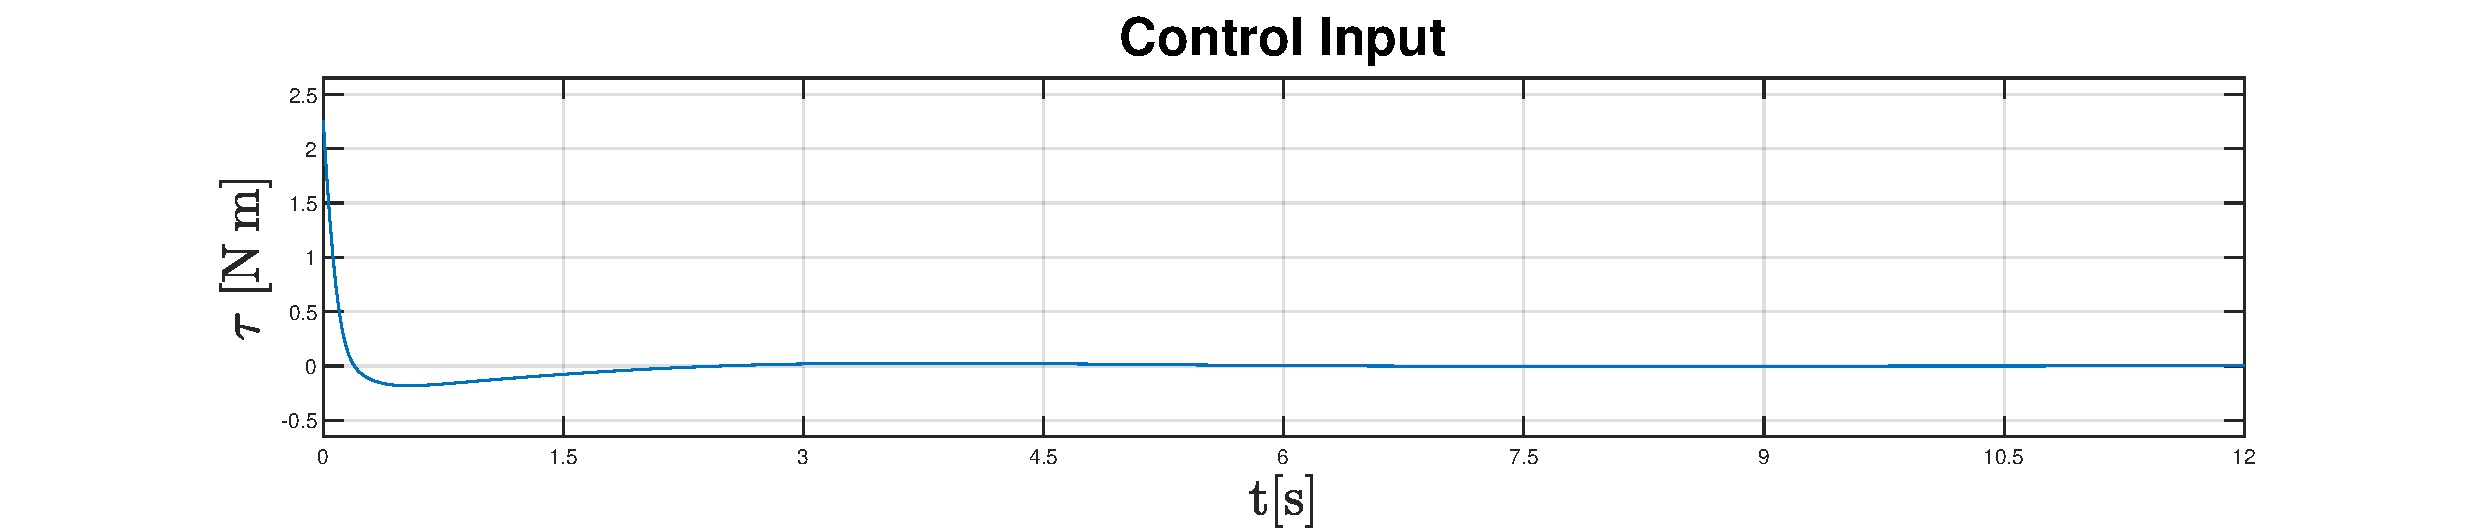
\includegraphics[scale=0.25]{images/MPC/control.pdf} 
		\end{subfigure}
	\end{figure}
\end{frame}

\begin{frame}
	\frametitle{Full-Range Control}	
	\begin{algorithm}[H]
		\caption{Heuristic Swing-Up Control strategy}
		\begin{algorithmic}[1]
			\Procedure{Heuristic Swing-Up Control}{}
			\State $\theta_1 \gets 180$ deg
			\State Pendulum is controlled by Energy-Shaping controller
			\If{$\theta_1 \in [-50,\;50]$ deg}		
			\State Pendulum is controlled by Predictive controller
			\EndIf
			\EndProcedure	
		\end{algorithmic}
	\end{algorithm}	
\end{frame}

\begin{frame}
	\frametitle{Full-Range Control}	
	\begin{figure}[H]
		\centering
		\begin{subfigure}
			\centering
			% include first image
			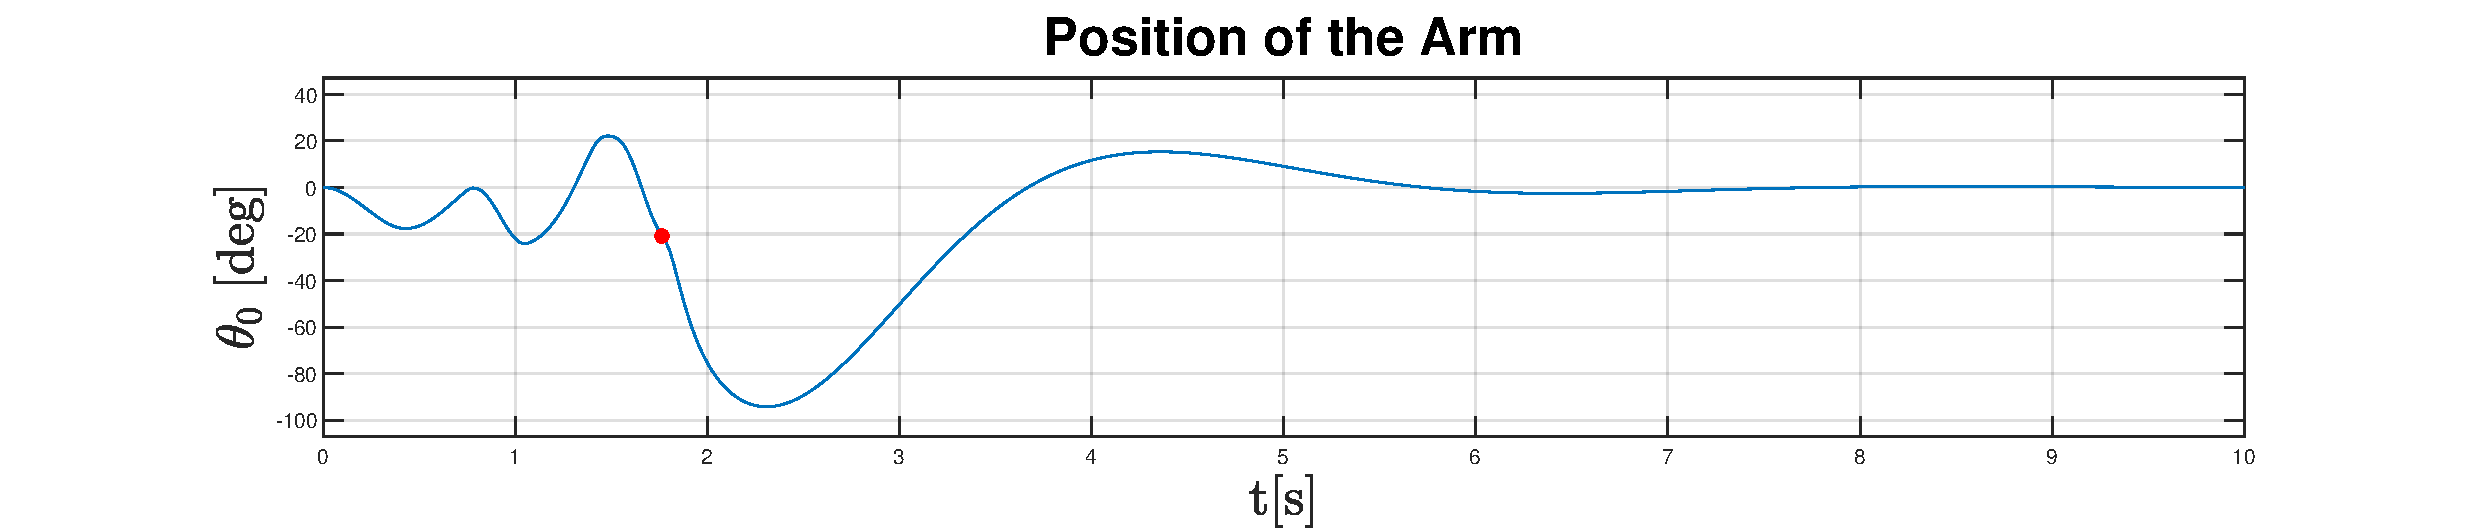
\includegraphics[scale=0.25]{images/Hswing/arm.pdf}  
		\end{subfigure}
		\begin{subfigure}
			\centering
			% include first image
			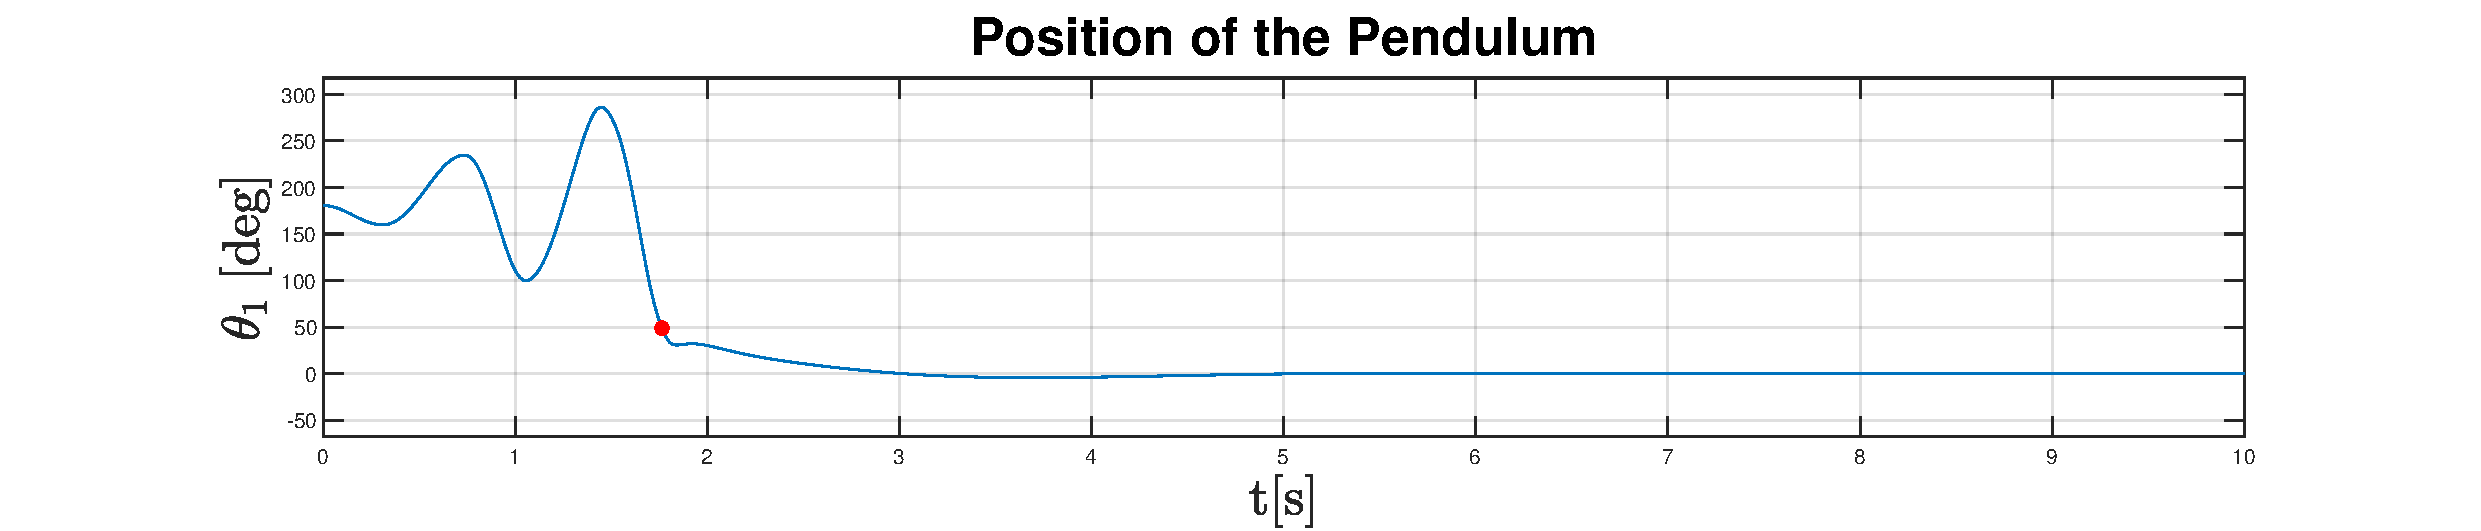
\includegraphics[scale=0.25]{images/Hswing/pend.pdf}  
		\end{subfigure}
		\begin{subfigure}
			\centering
			% include first image
			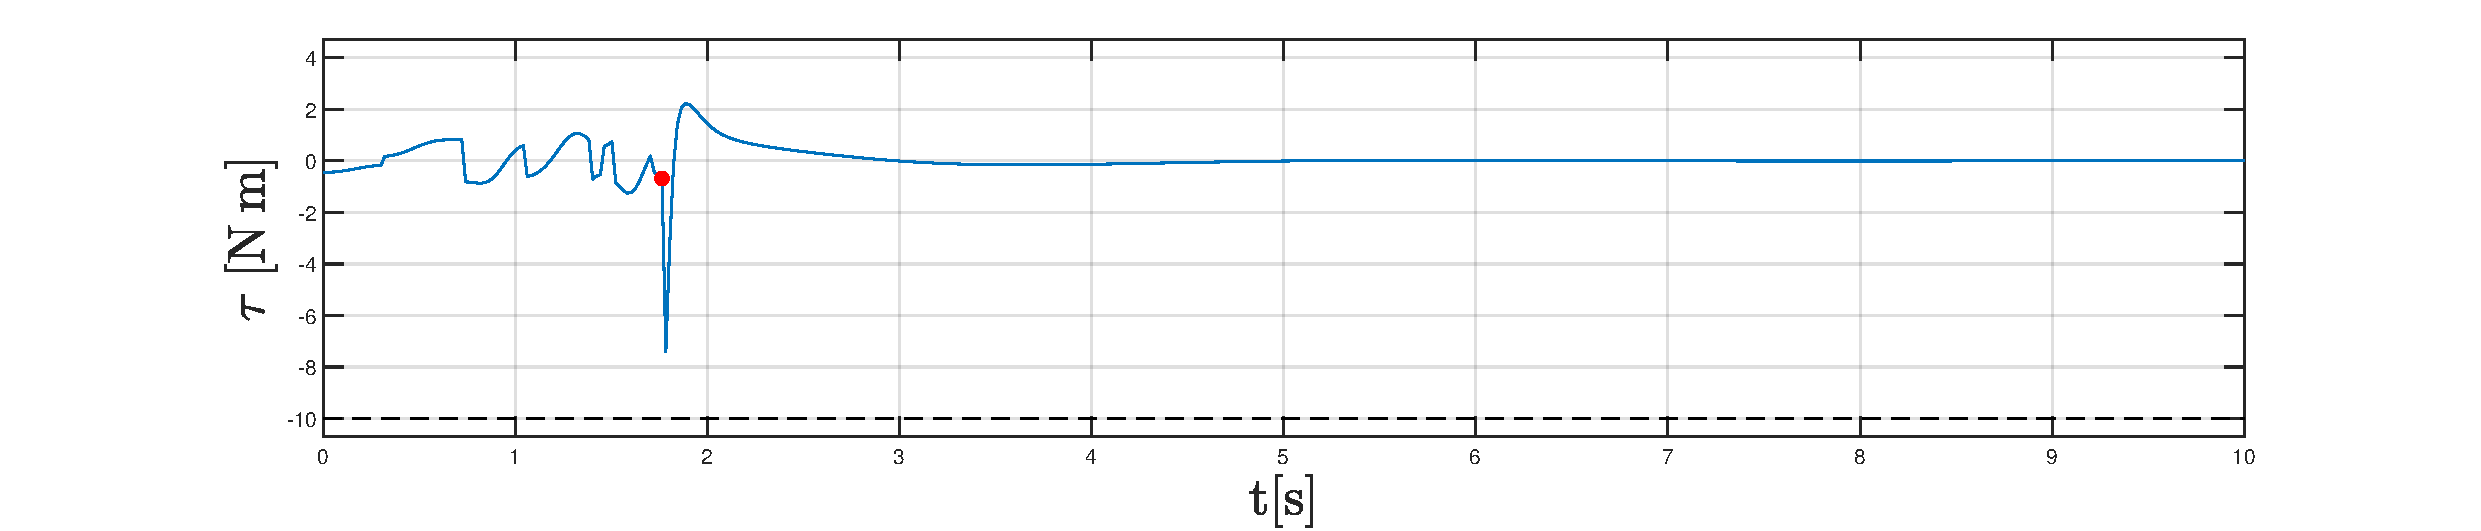
\includegraphics[scale=0.25]{images/Hswing/control.pdf} 
		\end{subfigure}
	\end{figure}
\end{frame}

\subsection{Optimal Swing-Up Control}
\begin{frame}
	\frametitle{Swing-Up Control of the Pendulum}	
	\begin{columns}[c]	
		\column{0.5\textwidth}
		Main control strategies
		\begin{enumerate}
			\item \textcolor{mygray}{Heuristic Swing-Up Control strategy}
			\item Optimal Swing-Up Control strategy\\			
		\end{enumerate}
		\column{0.4\textwidth}
		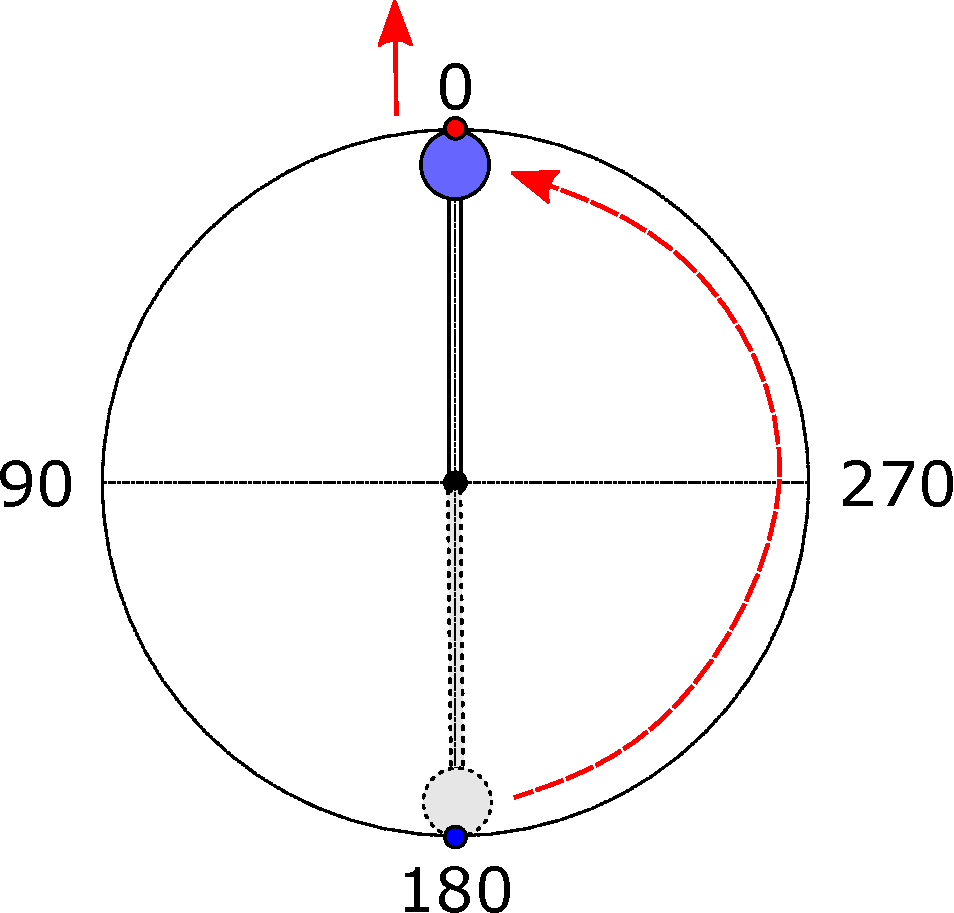
\includegraphics[scale=0.29]{images/OP_total.pdf}
	\end{columns}
\end{frame}
\begin{frame}
	\frametitle{Optimal Control Strategy}
		\vskip0.9em
		\begin{columns}[c]	
		\column{0.6\textwidth}
		Two phases of control:
	\begin{enumerate}
		\item Initial excitation of the system\\ (by Non-linear Predictive controller)\\
		\item Stabilisation of the pendulum\\(by Non-linear Predictive controller)
	\end{enumerate}
		\column{0.3\textwidth}
		\end{columns}
\end{frame}
\begin{frame}
	\frametitle{Non-Linerar Model Predictive Control}
	\phantom{Aa}
	\begin{subequations}
		\begin{align*}
		\min_{u_0,...,u_{N-1}}\ &\sum_{k=0}^{N-1} \lrp{ x_{k}^\intercal\ui{Q}{x}x_{k}^{\phantom{\intercal}}+u_{k}^\intercal\ui{Q}{u}u_{k}^{\phantom{\intercal}}}^{\phantom{\intercal}}\\
		\text{s.t.}\ &x_{k+1} = f(x_{k}, u_{k})\qquad\qquad\qquad \ \   k \in \mathbb{N}_0^{N-1}\\
		&\ui{u}{min}\leq u_{k}\leq \ui{u}{max}\qquad\qquad\qquad\;   k \in \mathbb{N}_0^{N-1}\\
		&x_0 = x(0)
		\end{align*}
	\end{subequations}
\small
\begin{table}[H]
	\begin{tabular}{l c c}
		\noalign{\hrule height 1pt}
		Parameter&Symbol&Value\\
		\noalign{\hrule height 1pt}
		Prediction horizon&$N$&$\ \; \,20$\\
		Initial condition&$x_0$&$\quad\begin{bmatrix}0\ 0\ 180\ 0\end{bmatrix}^\intercal$\\
		Constraint on control input-upper bound&$\ui{u}{max}$&$\ \; \,10$\\
		Constraint on control input-lower bound&$\ui{u}{min}$&$-10$\\
		\hline
	\end{tabular}
\end{table}
\newpage
\end{frame}
\begin{frame}
	\frametitle{Non-Linerar Model Predictive Control}
	\phantom{Aa}
	\begin{subequations}
		\begin{align*}
			\min_{u_0,...,u_{N-1}}\ &\sum_{k=0}^{N-1} \lrp{ x_{k}^\intercal\ui{Q}{x}x_{k}^{\phantom{\intercal}}+u_{k}^\intercal\ui{Q}{u}u_{k}^{\phantom{\intercal}}}^{\phantom{\intercal}}\\
			\text{s.t.}\ &x_{k+1} = f(x_{k}, u_{k})\qquad\qquad\qquad \ \   k \in \mathbb{N}_0^{N-1}\\
			&\ui{u}{min}\leq u_{k}\leq \ui{u}{max}\qquad\qquad\qquad\;   k \in \mathbb{N}_0^{N-1}\\
			&x_0 = x(0)
		\end{align*}
	\end{subequations}
Weight matrices
\begin{equation*}
\ui{Q}{x} = \begin{bmatrix}
1&0&0&0\\
0&0.1&0&0\\
0&0&3&0\\
0&0&0&0.1
\end{bmatrix} \quad \ui{Q}{u} = 0.1
\end{equation*}
\newpage
\end{frame}

\begin{frame}
	\frametitle{Full-Range Control}	
	Control of the arm
	\begin{figure}[H]
		\centering
		\begin{subfigure}
			\centering
			% include first image
			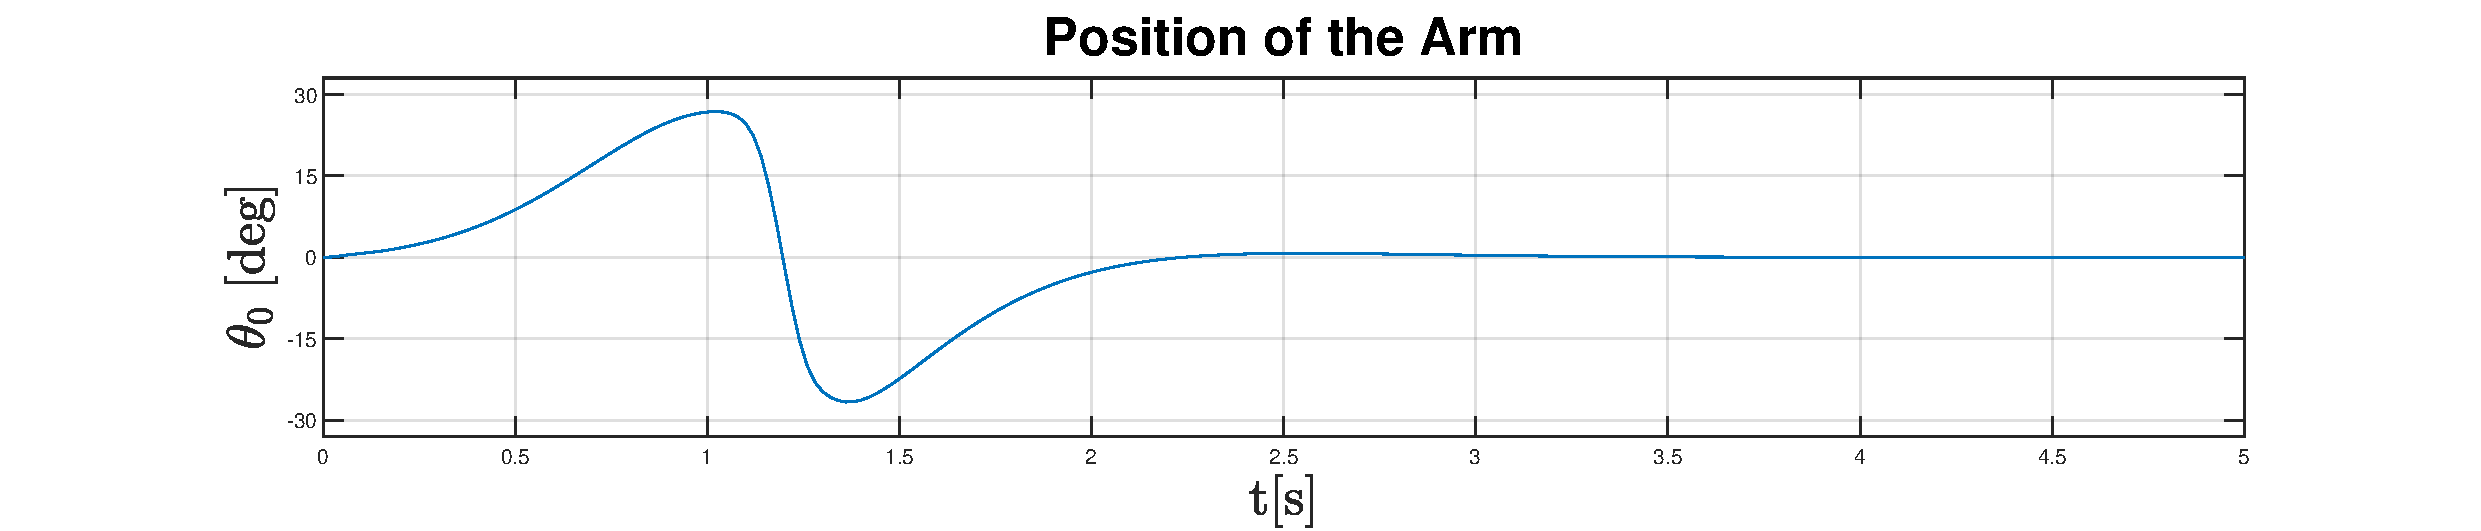
\includegraphics[scale=0.25]{images/Oswing/arm.pdf}  
		\end{subfigure}
		\begin{subfigure}
			\centering
			% include first image
			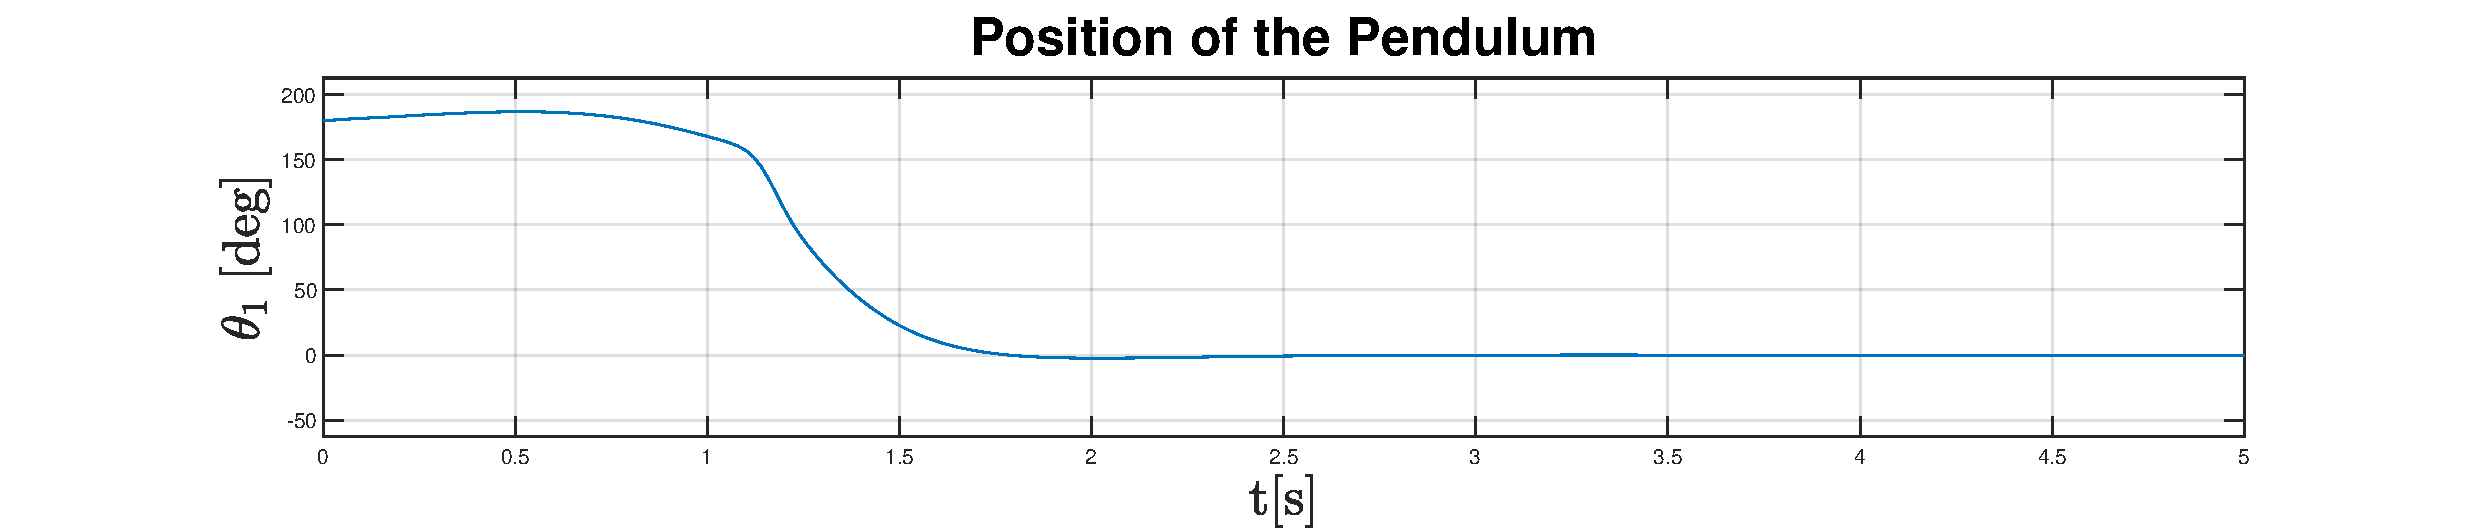
\includegraphics[scale=0.25]{images/Oswing/pend.pdf}  
		\end{subfigure}
		\begin{subfigure}
			\centering
			% include first image
			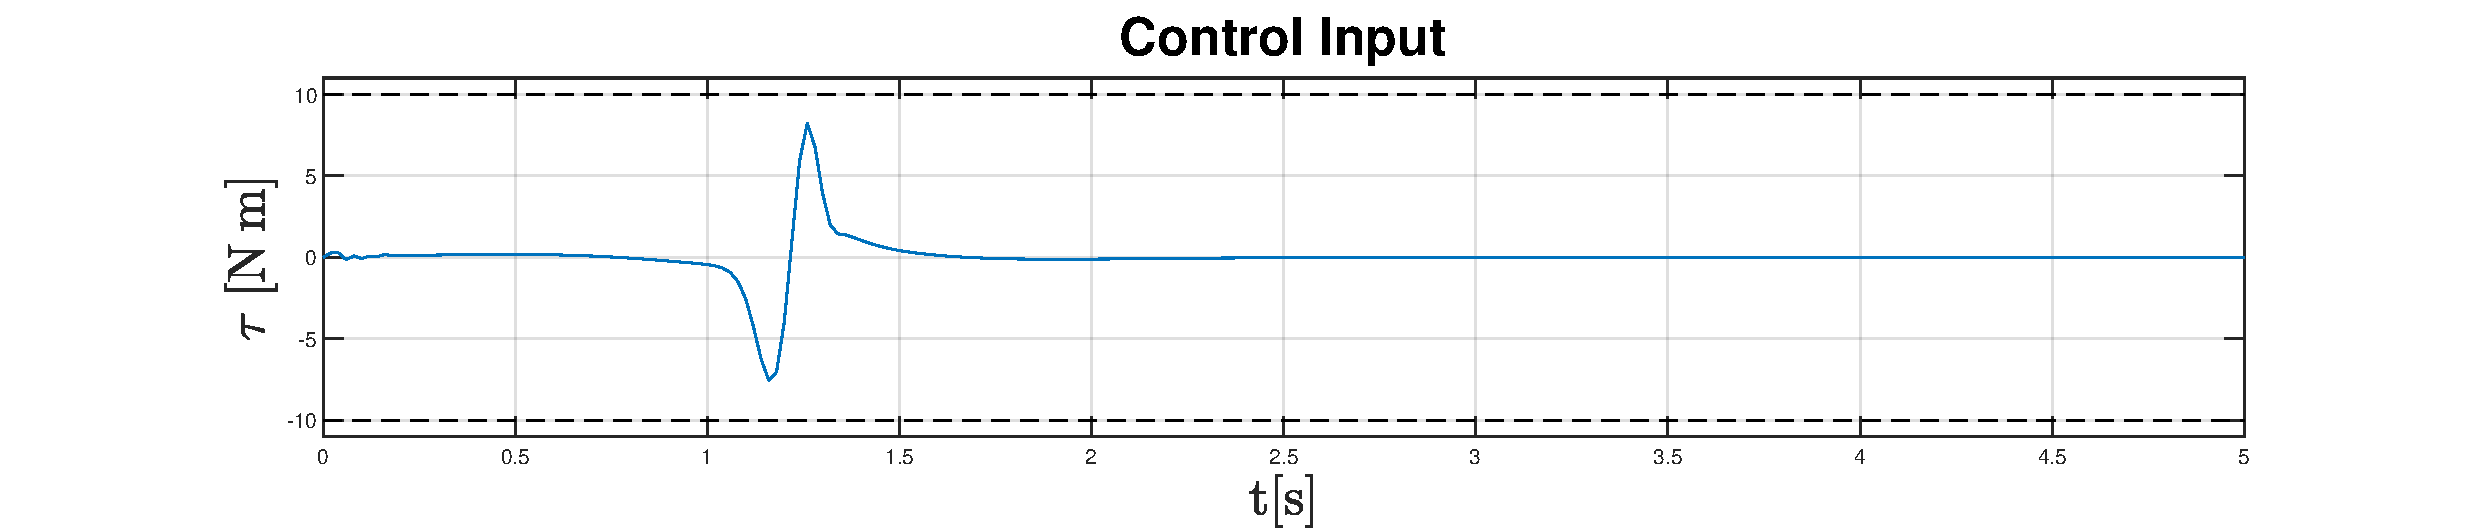
\includegraphics[scale=0.25]{images/Oswing/control.pdf} 
		\end{subfigure}
	\end{figure}
\end{frame}

\section{Conclusions}

\begin{frame}
	\frametitle{Discussion About Results}
	Quality criteria:
	\begin{itemize}
		\item Settling time\\
		\item Sum of abslolute error (SAE)\\
		\item Sum of squared control differences (SSCD)\\
		\item Solver solving time\\
	\end{itemize}
\end{frame}

\begin{frame}
	\frametitle{Discussion About Results}
	\begin{figure}[H]
		\begin{subfigure}
			\centering
			% include first image
			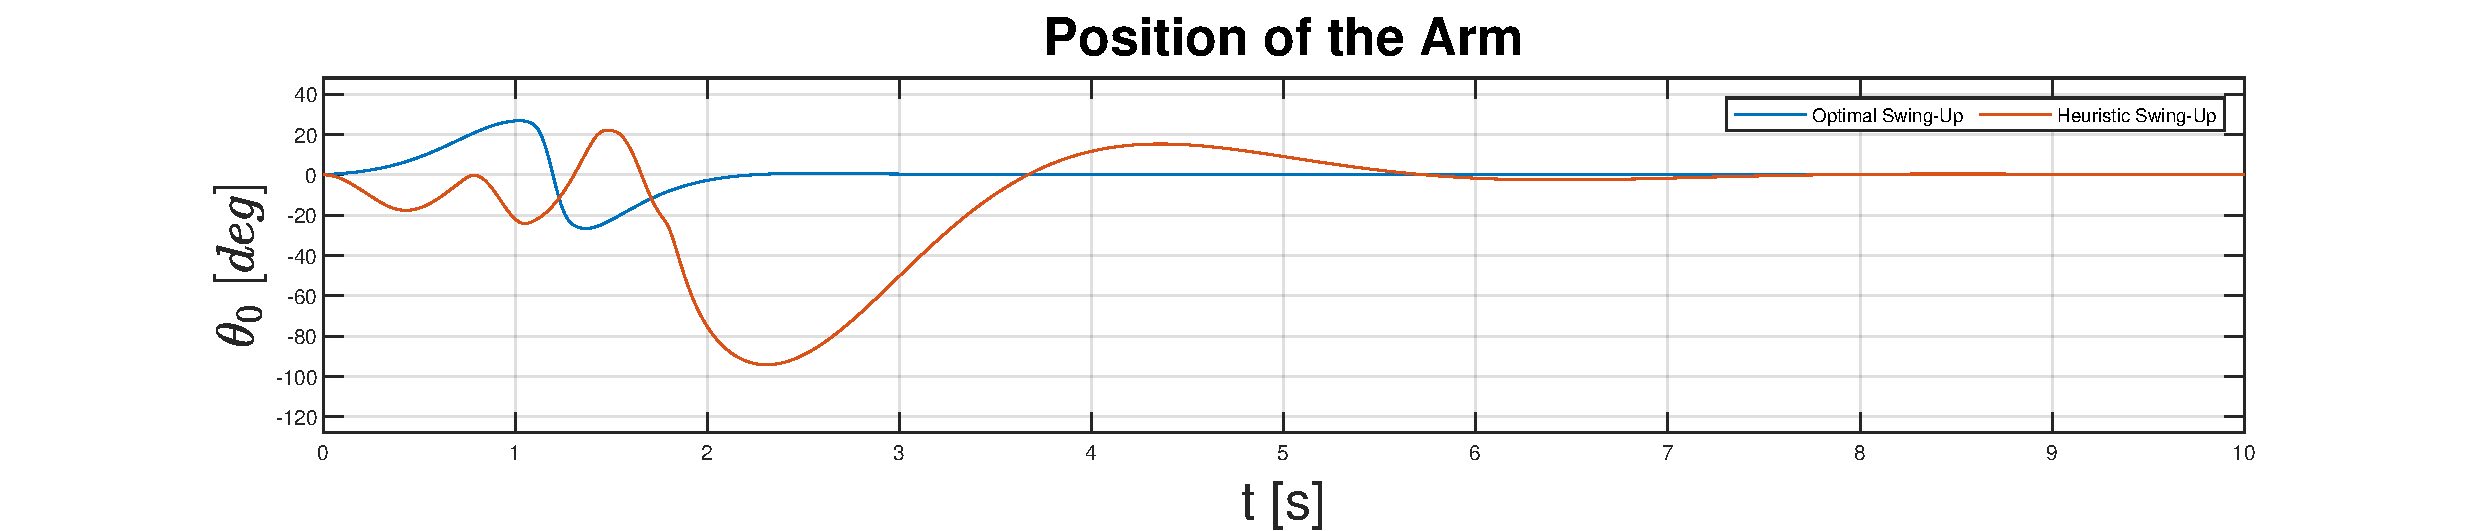
\includegraphics[scale=0.25]{images/Dswing/arm.pdf}  
		\end{subfigure}
		\begin{subfigure}
			\centering
			% include first image
			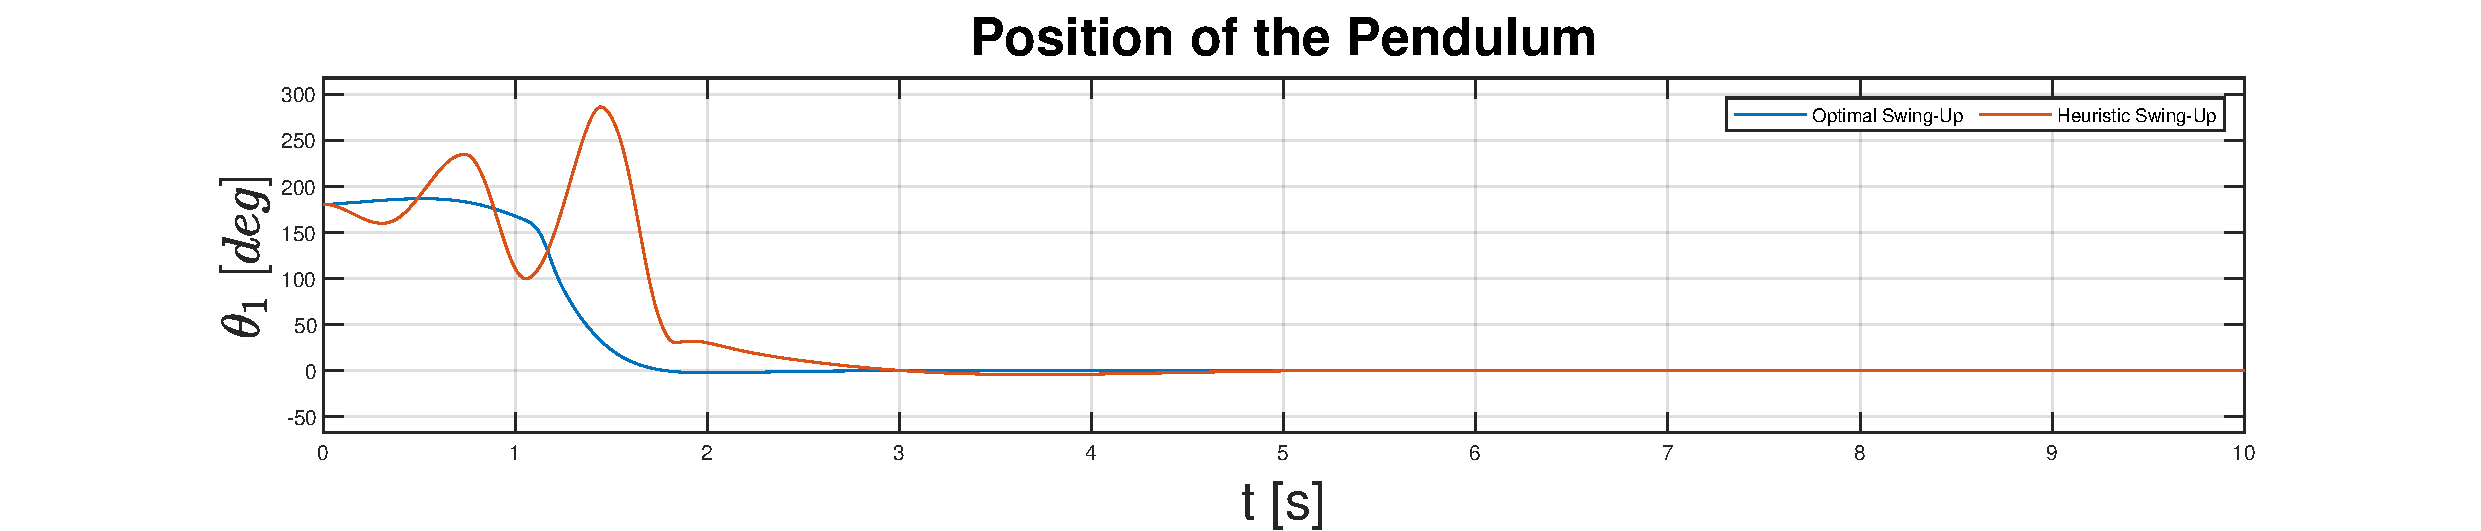
\includegraphics[scale=0.25]{images/Dswing/pend.pdf}  
		\end{subfigure}
		\begin{subfigure}
			\centering
			% include first image
			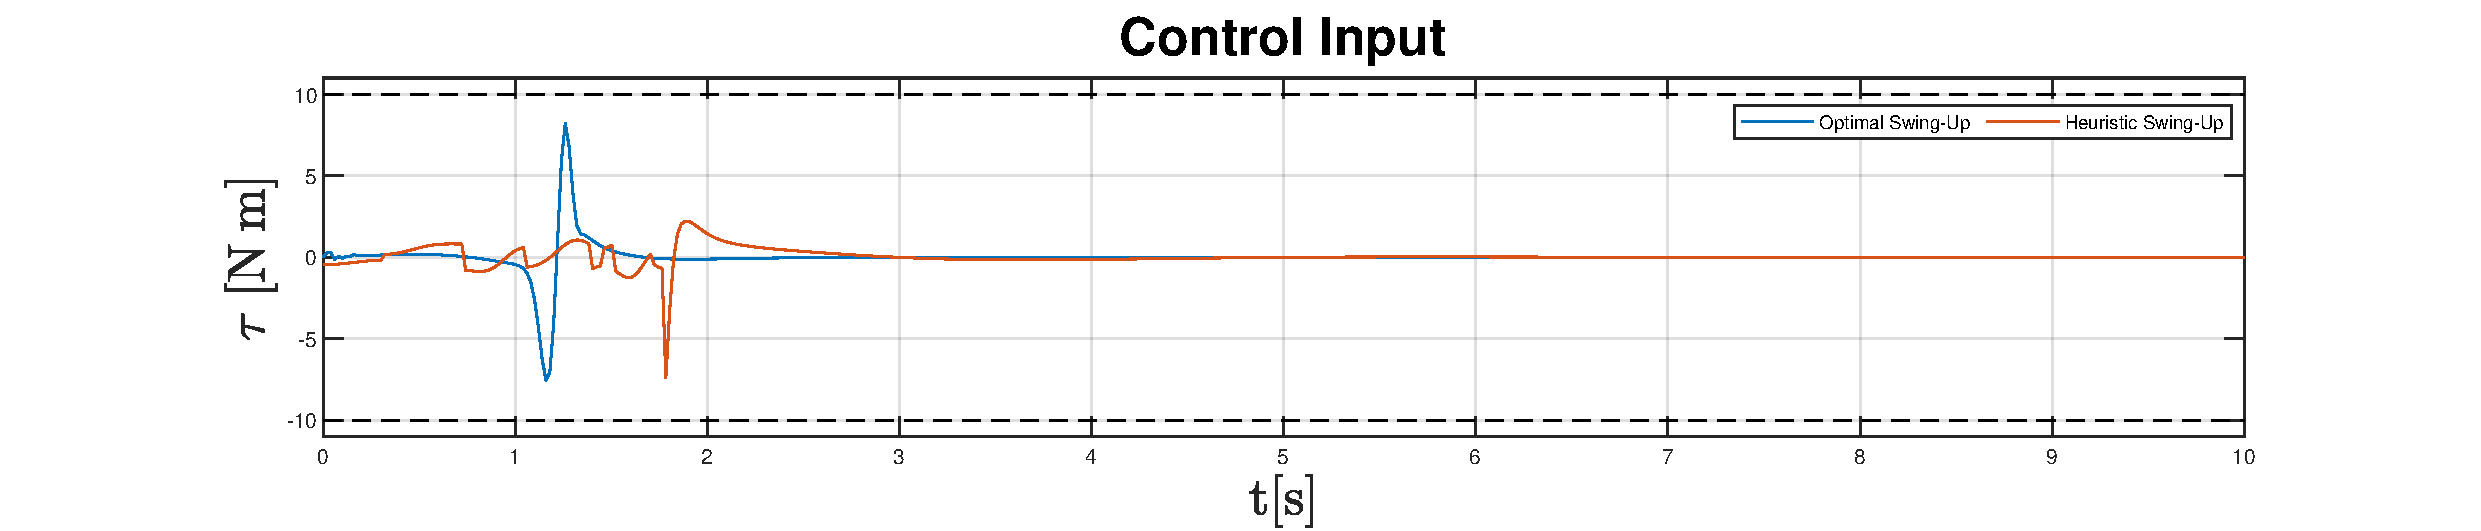
\includegraphics[scale=0.25]{images/Dswing/control.pdf} 
		\end{subfigure}
	\end{figure}
\end{frame}

\begin{frame}
	\frametitle{Discussion About Results}
	\begin{figure}[H]
	\begin{subfigure}
		\centering
		% include first image
		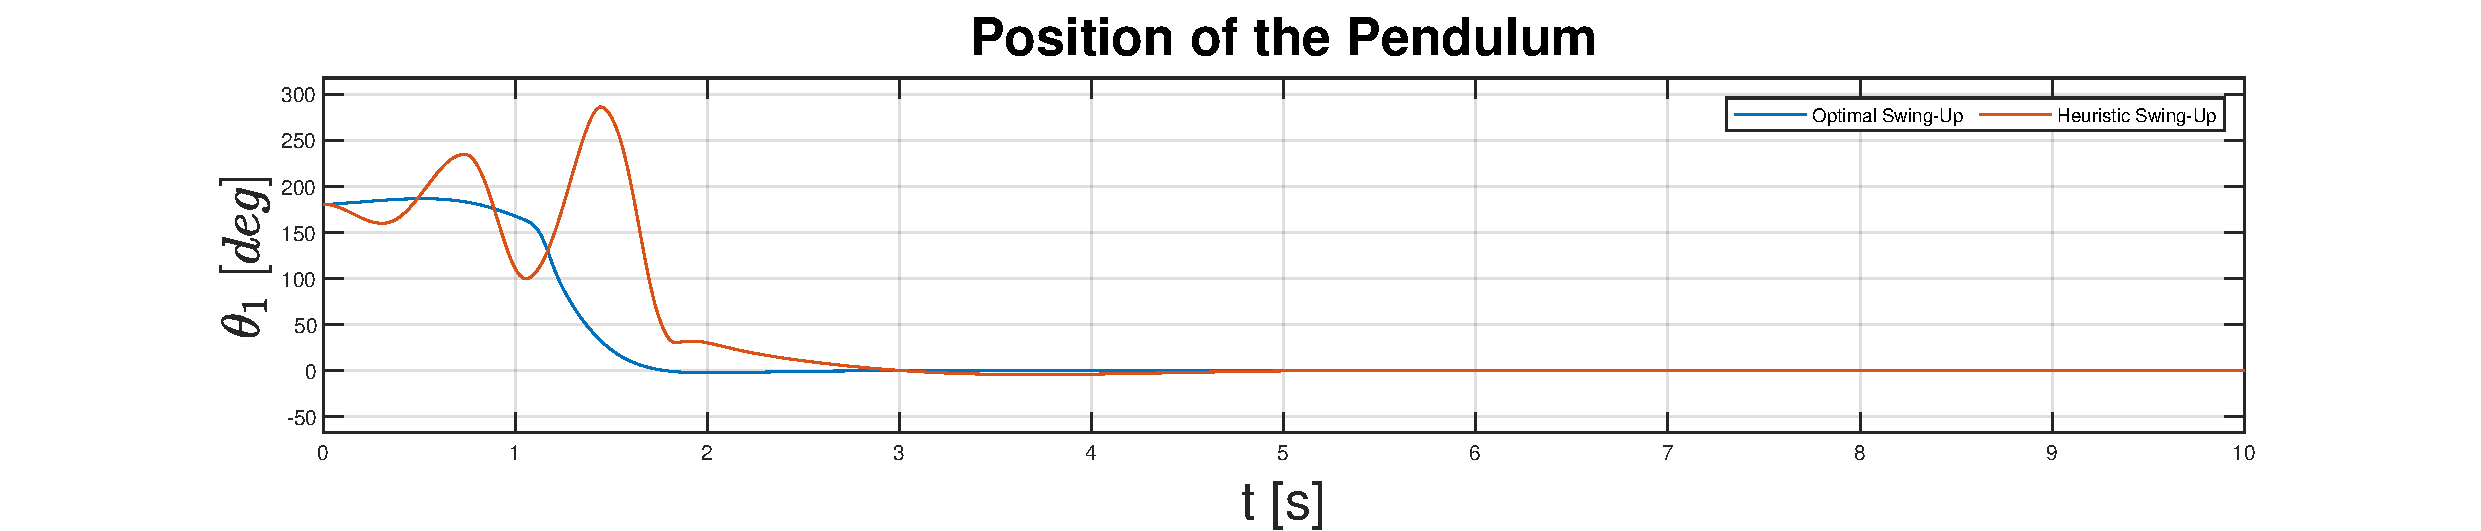
\includegraphics[scale=0.25]{images/Dswing/pend.pdf}  
	\end{subfigure}
	\begin{subfigure}
		\centering
		% include first image
		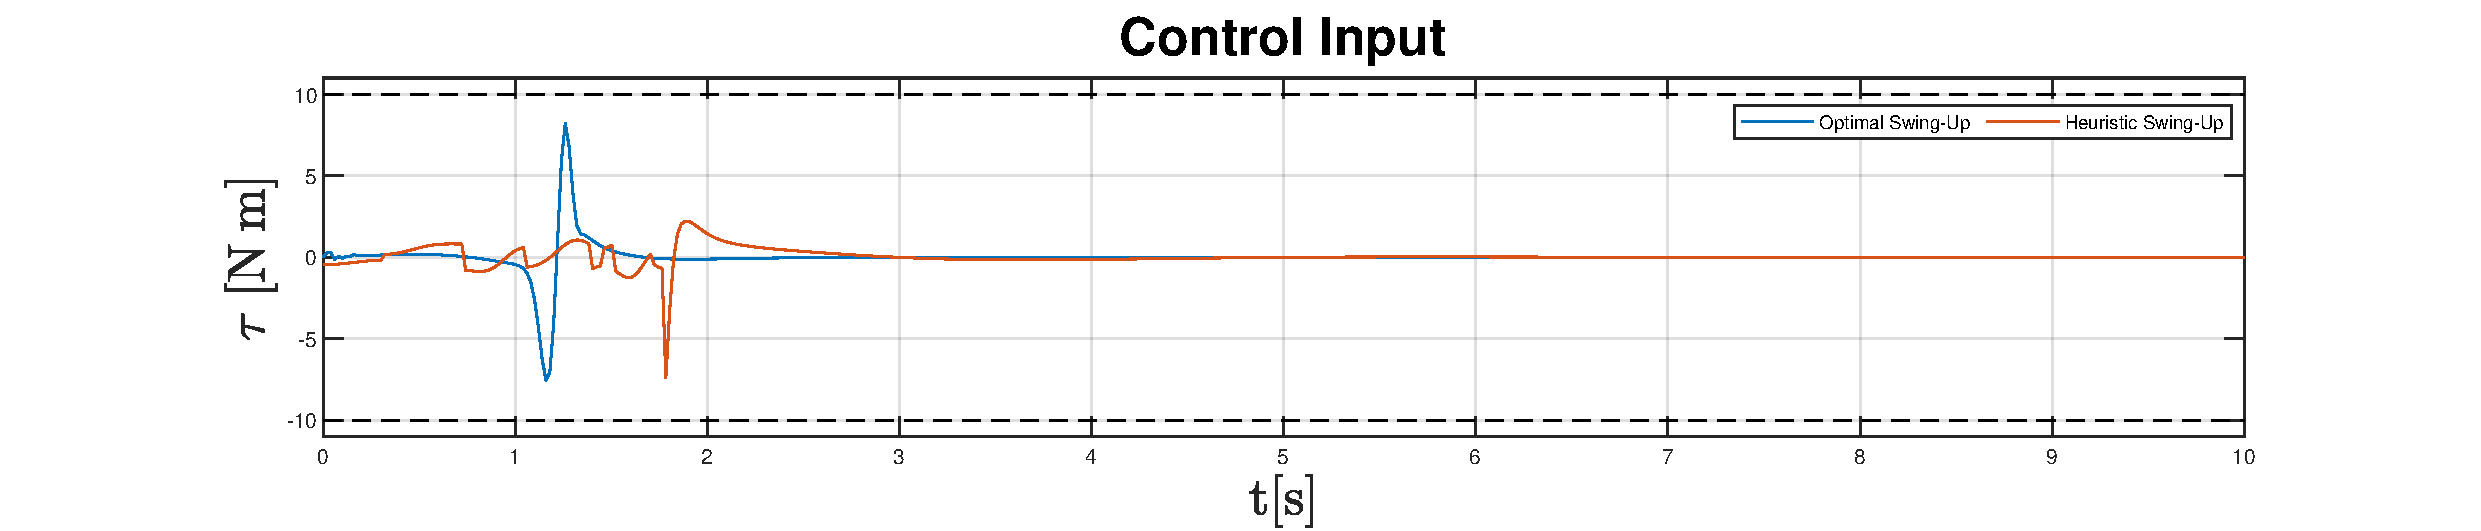
\includegraphics[scale=0.25]{images/Dswing/control.pdf} 
	\end{subfigure}
\end{figure}
	\begin{table}[H]
		\resizebox{\textwidth}{!}{
			\begin{tabular}{l c c c c c c}
				\noalign{\hrule height 1pt}
				\multirow{2}{*}{Strategy}&\multirow{2}{*}{Settling Time}&\multirow{2}{*}{SAE}&\multirow{2}{*}{SSCD}&\multicolumn{3}{c}{Solving Time}\\
				&&&&$\ui{t}{min}$&$\ui{t}{avg}$&$\ui{t}{max}$\\
				\noalign{\hrule height 1pt}
				Heuristic Swing-Up&7.51&305.15&86.77&0.0156&0.0234&0.0313\\
				Optimal Swing-Up&3.20&205.56&88.94&0.0313&0.0469&0.0625\\
				\hline
		\end{tabular}}
	\end{table}
\end{frame}

\begin{frame}
	\frametitle{Discussion About Results}
	\begin{figure}[H]
		\begin{subfigure}
	\centering
	% include first image
	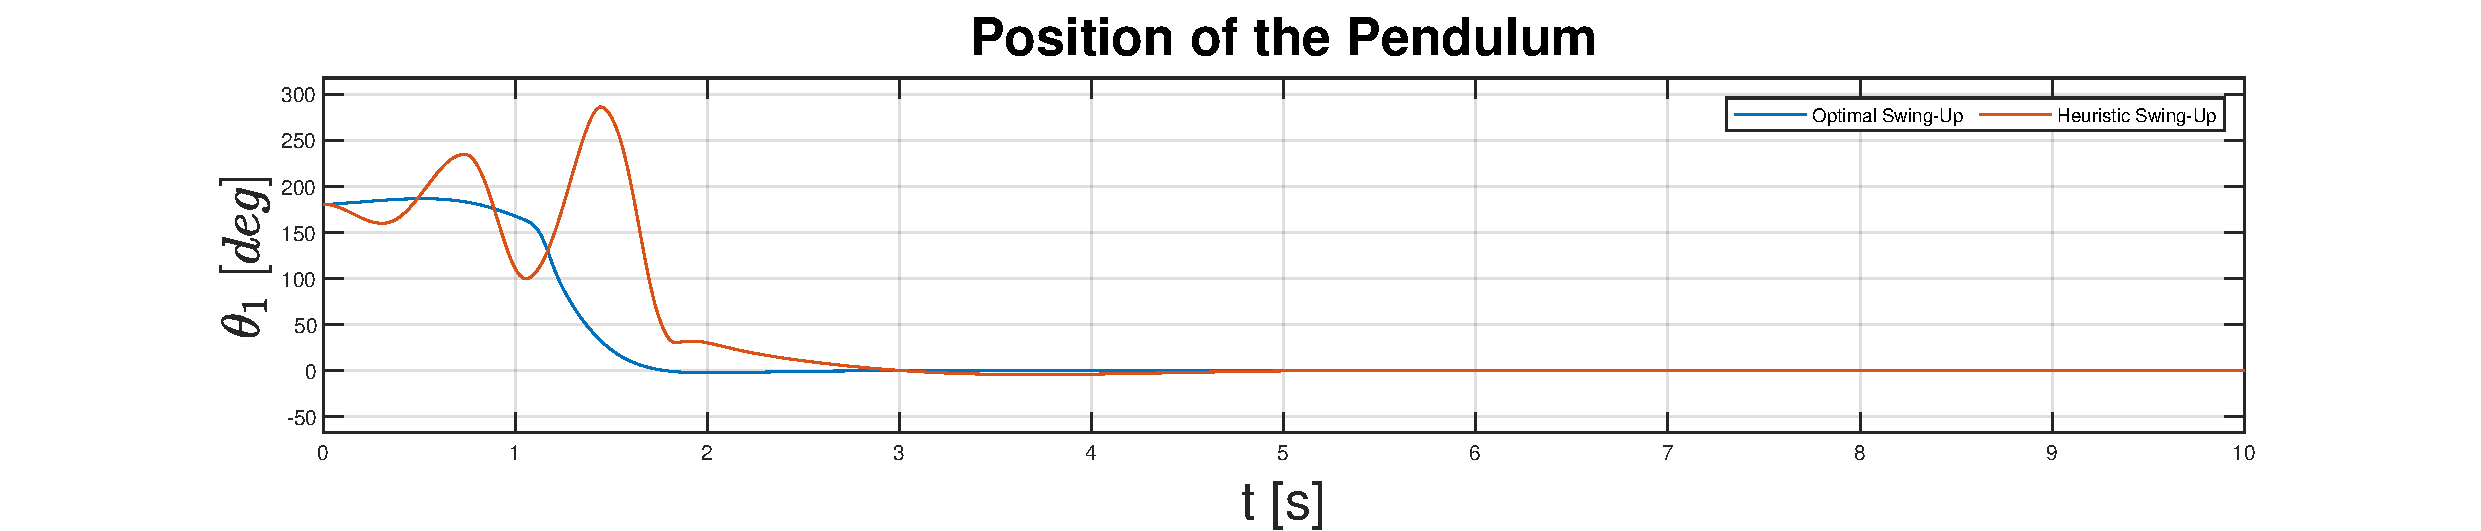
\includegraphics[scale=0.25]{images/Dswing/pend.pdf}  
\end{subfigure}
\begin{subfigure}
	\centering
	% include first image
	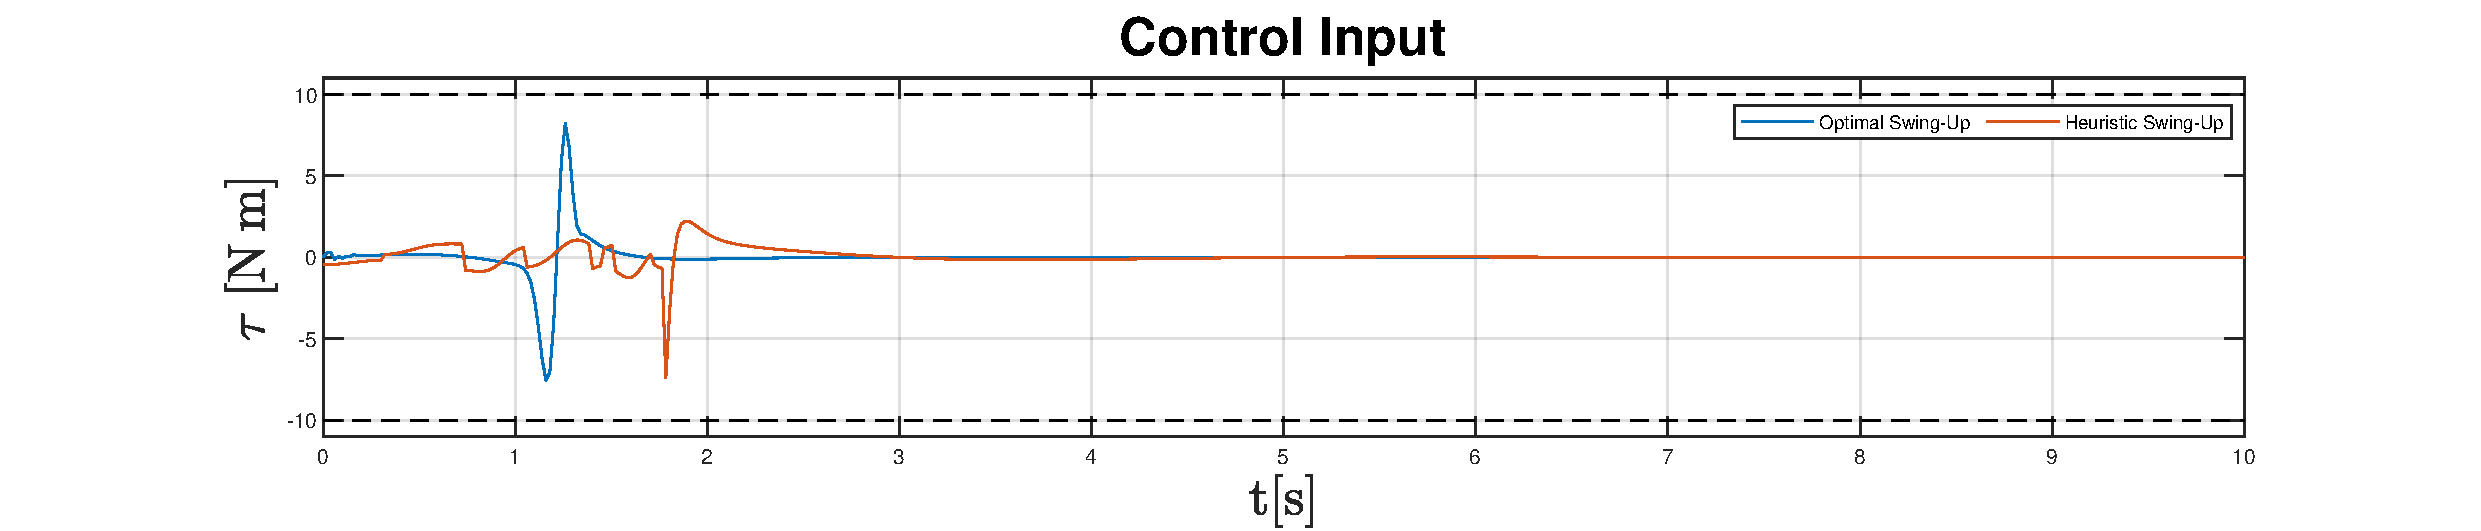
\includegraphics[scale=0.25]{images/Dswing/control.pdf} 
\end{subfigure}
\end{figure}
	\begin{table}[H]
		\resizebox{\textwidth}{!}{
			\begin{tabular}{l c c c c c c}
				\noalign{\hrule height 1pt}
				\multirow{2}{*}{Strategy}&\multirow{2}{*}{Settling Time}&\multirow{2}{*}{SAE}&\multirow{2}{*}{SSCD}&\multicolumn{3}{c}{Solving Time}\\
				&&&&$\ui{t}{min}$&$\ui{t}{avg}$&$\ui{t}{max}$\\
				\noalign{\hrule height 1pt}
				Heuristic Swing-Up&100\%&100\%&100\%&100\%&100\%&100\%\\
				Optimal Swing-Up&42.6\%&67.4\%&103\%&201\%&200\%&200\%\\
				\hline
		\end{tabular}}
	\end{table}
\end{frame}

\begin{frame}
	\frametitle{Summary}
	Main achievements of the thesis
	\begin{itemize}
	\item Design of Optimal Swing-Up control strategy\\
	\item Its comparisson against the heuristic method\\
	\item Evaluation of control quality and calculation time\\ of individual approaches
\end{itemize}
\end{frame}

\section{Backup}
\begin{frame}
	\frametitle{Parametres of the Pendulum}
	\begin{columns}[c]
		\column{2.3in}
		\centering
		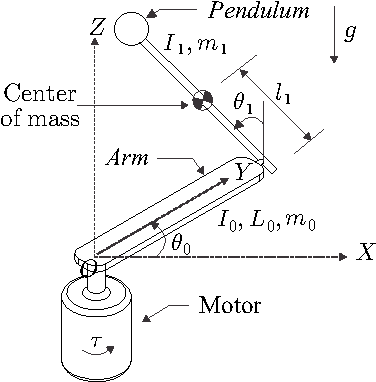
\includegraphics[scale=0.55]{images/furuta.png}
		\column{2.7in}  % slides are 3in high by 5in wide		
		\textit{g}-gravitational acceleration [ms$^{-2}$]\\
		\textit{m}$_0$-mass of arm [kg]\\
		\textit{m}$_1$-mass of pendulum [kg]\\
		\textit{L}$_0$-length of arm [m]\\
		\textit{L}$_1$-length of pendulum [m]\\
		\textit{l}$_0$-arms center of mass [m]\\
		\textit{l}$_1$-pendulums center of mass [m]\\
		\textit{I}$_0$-arms moment of inertia [kg m$^{-2}$]\\
		\textit{I}$_1$-pendulums moment of inertia [kg m$^{-2}$]\\
		$\theta_0$-arm angle[rad]\\
		$\theta_1$-pendulum angle [rad]\\
		$\tau$-motor torque [N m]\\		
	\end{columns}
\end{frame}
\end{document}
